\newchapter{phaseMons}{Phase Monitor Performance}

This is the introductory text.

Mon1 = first mon in CT
Mon2 = second mon in CT
Mon3 = mon in TBL

Mon1/Mon2 = upstream phase
Mon3 = downstream phase

\newsection{phaseMonDesign}{Phase Monitor Design}

Hybrid - remove dipole (position dependent) mode. 19dB below monopole mode for 1mm offset (11\% amplitude). 1mm beam offset = 2.8 degrees phase offset. 180 degree hybrids to remove. Additional 20 dB attenuation in dipole mode.

Bunch length sensitivity: more sensitive to variation in bunch length for longer variations. 5mm bunch length - 50\% amplitude output compared to 0mm. With 1mm bunches 16\% variation in bunch length needed to cause 1\% change in output voltage.

Mon1 24.6 dBm + 3dB
Mon2 26.8 dBm + 3dB
Mon3 24.5 dBm

\newsection{monElectronics}{Phase Monitor Electronics}


LO should have 5fs stability? What is the source of the LO?

Mixer output
\begin{align}
RF(t) &= A_{RF}(t)\cos[\omega_{RF} t + \phi(t)] \\
LO(t) &= A_{LO}\cos[\omega_{LO} t]
\end{align}
mixer multiplies
\begin{align}
\mathrm{Mixer}(t) &= RF(t) \times LO(t) \\
\mathrm{Mixer}(t) &= A_{RF}(t)A_{LO}\cos[\omega_{RF} t + \phi(t)]\cos[\omega_{LO} t]
\end{align}
trig identities
\begin{equation}
\mathrm{Mixer}(t) = \frac{A_{RF}(t)A_{LO}}{2}\left\lbrace\cos[(\omega_{LO} + \omega_{RF})t + \phi(t)] + \cos[(\omega_{LO} - \omega_{RF})t + \phi(t)]\right\rbrace
\end{equation}
filter high frequency
\begin{equation}
\mathrm{Mixer}(t) = \frac{A_{RF}(t)A_{LO}}{2}\cos[(\omega_{LO} - \omega_{RF})t + \phi(t)]
\label{e:mixOutAnyFreq} 
\end{equation}
LO frequency and RF frequency are the same
\begin{equation}
\mathrm{Mixer}(t) = \frac{A_{RF}(t)A_{LO}}{2}\cos[\phi(t)]
\label{e:mixOutSameFreq} 
\end{equation}
Diode used to measure \(A_{RF}\)
\begin{equation}
\mathrm{Diode}(t) = A_{RF}(t)^2
\label{e:idealDiode}
\end{equation}
The phase can be reconstructed by
\begin{align}
&\frac{\mathrm{Mixer}(t)}{\sqrt{\mathrm{Diode}(t)}} = A\cos[\phi(t)] \label{e:mixOverSqrtDio} \\
&\phi(t) = \arccos\left[\frac{\mathrm{Mixer(t)}}{A\sqrt{\mathrm{Diode(t)}}}\right]
\label{e:phaseRecIdeal} 
\end{align}

Beam/monitor frequency is 11.994 GHz.

Performance limited by:
Device non-linearity -- normally better for lower input power
Signal to noise -- better for high power
Therefore, split signal to 8 mixers -- low input power to each one -- to reduce effect of non-linearities. Then sum up results of each mixer to improve signal to noise.

Monitor -> attenuator? -> Hybrid sum -> attenuator? -> attenuator in gallery -> mixer RF input
LO -> phase shifter -> multiplier -> amplifier -> mixer LO input
Mixer output -> attenuator -> amplifier -> SiS OR -> attenuator->FONT
Diode output -> SiS/FONT

Latest power measurements:

LO1 22.6 dBm
LO2 23.6 dBm
LO3 25.5 dBm

\newsection{s:resolutionEqs}{Resolution Definition}

The performance of the PFF system clearly depends on the accuracy to which the phase can be measured. Many of the measurements in this chapter are therefore focused on the phase monitor resolution, or more precisely on the resolution of the combined phase monitor and electronics setup. The resolution is defined as the jitter between the measured phase and the true beam phase. This can be calculated by comparing the difference between the measured phase of two monitors. This is why two phase monitors, Mon~1 and Mon~2 are installed neighbouring each other in the upstream system in the CT line. The beam phase should be identical in these two monitors thus their measurements can always be compared to derive the resolution.

The precise derivation of the resolution dependent on the measurement of two monitors is as follows. First, the measured phase, \(\phi_x(t)\) and \(\phi_y(t)\), in two monitors at time \(t\) can be defined as:
\begin{align}
\phi_x(t) &= \phi_b(t) + n_x(t) \\
\phi_y(t) &= \phi_b(t) + n_y(t)
\end{align}
Where \(\phi_b(t)\) is the true beam phase and \(n_x(t)\) and \(n_y(t)\) is the noise on the measurement at that time. The time dependence will not be written explicitly from this point. These equations assume the beam phase is identical in each monitor, as should be the case for Mon~1 and Mon~2. The variance of each phase monitor measurement can then be derived from the equations above by adding the variance of the beam phase and the noise in quadrature:
\begin{align}
\sigma_x^2 &= \sigma_b^2 + \sigma_{nx}^2 \\
\sigma_y^2 &= \sigma_b^2 + \sigma_{ny}^2
\end{align}
Where \(\sigma_x\) and \(\sigma_y\) are the phase jitters measured by each phase monitor, \(\sigma_b\) is the true beam phase jitter and \(\sigma_{nx}\) and \(\sigma_{ny}\) are the phase monitor resolutions. Assuming each phase monitor has the same resolution, \(\sigma_n\), this can be simplified to \(\sigma_x^2~=~\sigma_y^2~=~\sigma_b^2~+~\sigma_n^2\).

The quantity of interest for calculating the phase monitor resolution is the jitter in the difference between the two measured phases, \(\sigma_{x-y}\). The variance of the difference between two correlated variables is defined as:
\begin{align}
\sigma_{x-y}^2 &= \sigma_x^2 + \sigma_y^2 - 2\sigma_x\sigma_y\rho_{xy} \\
\end{align}
Where \(\rho_{xy}\) is the correlation between the phase measurement of \(x\) and \(y\). Substituting in the previously derived expressions for \(\sigma_x\) and \(\sigma_y\) this becomes:
\begin{align}
\sigma_{x-y}^2 &= 2(\sigma_b^2 + \sigma_n^2)(1-\rho_{xy})
\end{align}

The correlation coefficient \(\rho_{xy}\) depends on the covariance between \(x\) and \(y\), \(\mathrm{cov}[x,y]\), as follows:
\begin{align}
\rho_{xy} &= \frac{\mathrm{cov}[x,y]}{\sigma_x\sigma_y} = \frac{\mathrm{cov}[x,y]}{\sigma_b^2+\sigma_n^2} \\
\end{align}
Where the covariance is defined as:
\begin{align}
\mathrm{cov}[x,y] = \frac{1}{N}\sum_{i=1}^{N}\phi_{xi}\phi_{yi} \\
\end{align}

Substituting in the expressions for \(\phi_{x}\) and \(\phi_{y}\) above and separating the terms in the sum then gives the following expression for the covariance of \(x\) and \(y\):
\begin{equation}
\begin{gathered}
\mathrm{cov}[x,y] = \frac{1}{N}\sum_{i=1}^{N}(\phi_{bi}+n_{xi})(\phi_{bi}+n_{yi}) \\
\mathrm{cov}[x,y] = \frac{1}{N}\sum_{i=1}^{N}\phi_{bi}^2 + \frac{1}{N}\sum_{i=1}^{N}\phi_{bi}n_{xi} + \frac{1}{N}\sum_{i=1}^{N}\phi_{bi}n_{yi} + \frac{1}{N}\sum_{i=1}^{N}n_{xi}n_{yi} 
\end{gathered}
\end{equation}
The first term is the definition of the variance of the beam phase, \(\sigma_b^2\). The remaining terms are the covariance between the beam phase and the monitor noises, and the covariance between the two monitor noises. Assuming the noise is uncorrelated all these terms are zero. The remaining equation for the covariance between \(x\) and \(y\) is therefore simply: \(\mathrm{cov}[x,y] = \sigma_b^2\). Finally, the correlation between the phase measurement of \(x\) and \(y\) becomes:
\begin{align}
\rho_{xy} &= \frac{\sigma_b^2}{\sigma_b^2 + \sigma_n^2}
\label{e:corrVsResolution}
\end{align}

Substituting this expression for the correlation in to the derived equation for the variance between the two phase measurements gives the following simple dependence on the phase monitor resolution:
\begin{equation}
\begin{gathered}
\sigma_{x-y}^2 = 2(\sigma_b^2 + \sigma_n^2)\left(1-\frac{\sigma_b^2}{\sigma_b^2 + \sigma_n^2}\right) \\
\sigma_{x-y}^2 = 2\sigma_n^2 \label{e:pffVsResolution}
\end{gathered}
\end{equation}
Finally, the resolution is defined as:
\begin{align}
\sigma_n = \frac{\sigma_{x-y}}{\sqrt{2}}
\label{e:resolutionEq}
\end{align}
In terms of a resolution calculation these equations only apply to the two upstream phase monitors. All the resolution values quoted in this chapter use this equation and the difference between the measurement of Mon~1 and Mon~2.

However, as the act of the PFF system can also be thought of as subtracting two phases (removing the upstream phase from the downstream phase) the same equations can be directly applied to determine the limitations that the phase monitor resolution places on the PFF performance. Equation~\ref{e:pffVsResolution} shows that the lowest possible corrected downstream phase jitter is a factor \(\sqrt{2}\) times larger than the phase monitor resolution. In order to reduce the downstream phase jitter to the CLIC target of \(0.2^\circ\) the phase monitor resolution must therefore be better than \(0.14^\circ\). Equation~\ref{e:corrVsResolution} shows that with this \(0.14^\circ\) resolution and a typical beam phase jitter of \(0.8^\circ\) (Section~\ref{s:origJitter}) the measured correlation between two phase monitor measurements would be \(97\%\).

\newsection{monDigitisers}{Digitisation of Phase Monitor Signals}

The mixer and diode outputs from the phase monitor electronics must be digitised on analogue to digital converters (ADCs) so the signals can be processed and used for the PFF correction and offline data analysis. Two different types of ADCs have been used to digitise the phase monitor signals --- the Texas Instruments ADS5474 ADCs [REF] on the purpose-built FONT5a board used as the PFF controller and a commercially available SiS 3320 digitiser [REF]. The design and use of the FONT5a board is discussed in more detail in Section~\ref{s:fontSetup}. Table~\ref{t:adcSpecs} summarises the specifications of each type of ADC. 

The SiS digitisers are used in addition to the FONT5a board as the PFF correction running on the FONT5a board is operated as a standalone system independent from other acquisition systems at CTF3. The PFF algorithm requires only the signals from one of the upstream phase monitors to be connected to the FONT5a board, with the convention being to use Mon~1. Mon~2 and Mon~3 are then normally connected to the SiS digitisers instead. The SiS digitisers are setup with the same trigger and sampling frequency (192~MHz) used for other signals at CTF3, and data from them can be acquired together with other devices using the standard systems in place at CTF3. This allows the Mon~2 and Mon~3 signals to be easily compared to other measurements, such as beam position signals, which has been indispensable for optimising the setup of the PFF system and in particuar the phase propagation (Chater~\ref{c:phasePropagation}).

\begin{table}
  \begin{center}
    \begin{tabular}{|c c c c c c|}
	   \hline
       Digitiser & No. ADCs & Resolution & Input Range & Sampling Rate & Bandwidth \\ \hline
       SiS 3320 & 8 & 12-bit & \(\pm2.5\)~V & up to 250~MHz & 100~MHz\\
       FONT5a & 9 & 14-bit (13-bit used) & \(\pm0.5\)~V & up to 400~MHz & 1.4~GHz\\ \hline
    \end{tabular}
    \caption{Specifications of the ADCs on the FONT5a board and SiS digitisers.}
  	\label{t:adcSpecs}
  \end{center}
\end{table}

Digitising the phase monitor signals contributes additional noise to the overall phase monitor electronics setup. The purpose of this section is to ensure that the digitiser noise makes only a negligible contribution to the resolution on the phase measurement. The main parameters of interest needed to determine this are the input range and resolution of the ADCs, with the SiS ADCs being 12-bit with a range of \(\pm2.5\)~V and the FONT5a ADCs being 13-bit with an input range of \(\pm0.5\)~V. The full 5~V peak-to-peak input range of the SiS ADCs is therefore split across \(2^{12}=4096\) values, or ADC `counts', with each count corresponding to roughly 1.2~mV. The equivalent 1~V peak-to-peak range and \(2^{13}=8192\) counts of the FONT5a board corresponds to a factor 10 lower interval of 0.12~mV per ADC count. The voltage jitter added by the digitisation of the phase monitor signals cannot be expected to be better than 1~count. This already indicates that the FONT5a board should give a much lower contribution to the phase resolution than the SiS digitisers.

Figure~\ref{f:digitiserNosie} shows the ADC noise, converted from counts in to an equivalent voltage, for both the SiS and FONT5a ADCs. As expected the noise on the FONT5a board is much lower than on the SiS digitisers. The actual ADC jitter values are \(1.47\pm0.04\)~counts or \(0.179\pm0.005\)~mV on the FONT5a board, and \(1.11\pm0.03\)~counts or \(1.36\pm0.03\)~mV on the SiS digitisers. These values can be converted in to an equivalent phase jitter using the phase reconstruction method described later in Section~\ref{ss:sigGenConsq} and the monitor calibration constants determined in Section~\ref{s:monCalibrations}. For reference the peak output of the three phase monitor mixers varies between approximately 400~mV and 500~mV, which is well matched to the input range of the FONT5a ADCs. Taking the worst case scenario of Mon~3, which gives the lowest output voltage, the ADC jitter corresponds to \(0.0245\pm0.0007^\circ\) on the FONT5a board but \(0.198\pm0.005^\circ\) on the SiS digitisers. These values are summarised in Table~\ref{t:adcNoise}.

\begin{figure}
  \centering
  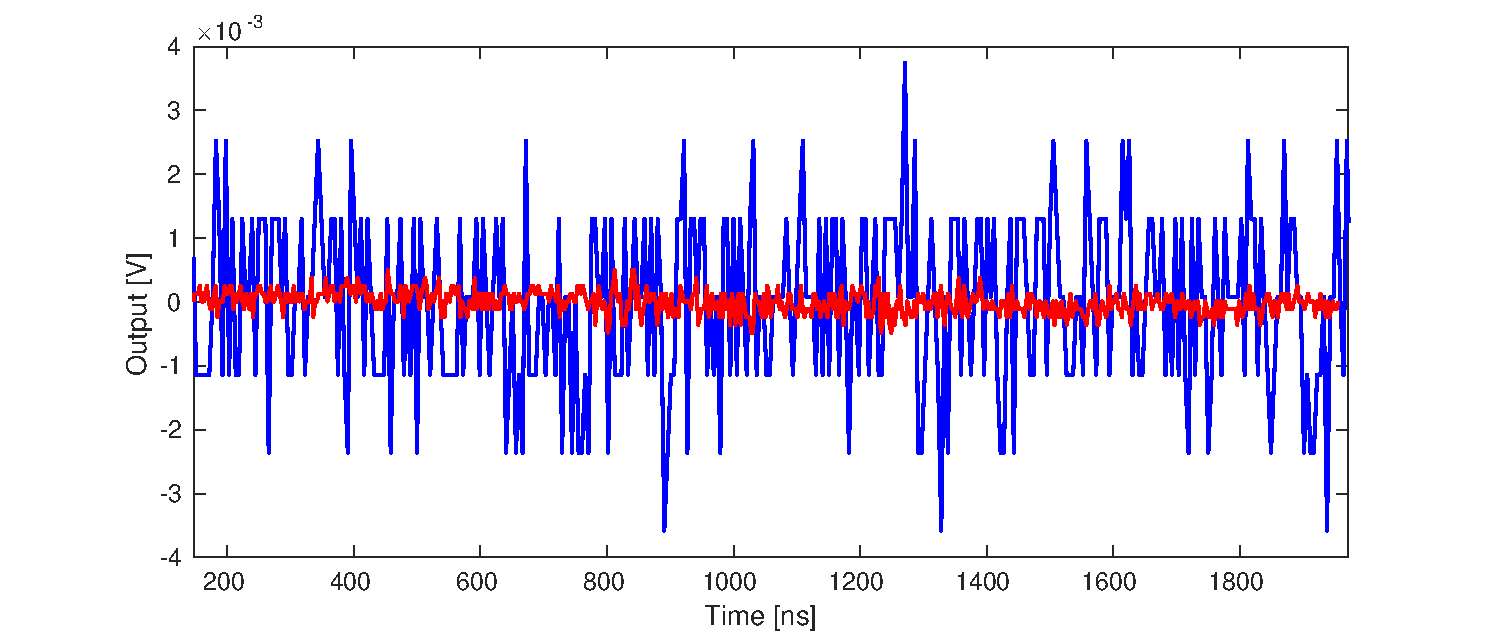
\includegraphics[width=0.9\textwidth]{Figures/phaseMons/digitiserNosie}
  \caption{Comparison of noise on the output of the SiS and FONT5a ADCs.}
  \label{f:digitiserNosie}
\end{figure}

As derived in the previous section the phase resolution must be better than \(0.14^\circ\) in order to achieve a corrected downstream phase jitter of \(0.2^\circ\) with the PFF system. The \(\sim0.02^\circ\) contribution of ADC noise on the FONT5a board is therefore insignificant compared to the resolution requirements. However, although it does not directly impact the PFF performance the \(\sim0.2^\circ\) ADC jitter on the SiS digitisers would greatly degrade the resolution of the measurements of Mon~2 and Mon~3 usually connected to the SiS~digitisers and used for offline data analysis of the PFF results. 

The high phase jitter contribution from the SiS digitisers originates from the roughly 500~mV maximum mixer output being much lower than the SiS ADC range of \(\pm2.5\)~V. In order to rectify this the mixer outputs are boosted by roughly a factor 2.5 in voltage using an amplifier prior to the SiS digitisers. The specifications of the amplifier used are documented in [REF]. With the amplifier in place the peak signal level sent to the SiS digitisers is around 1~V, and the equivalent phase jitter is reduced to \(0.078\pm0.002^\circ\). This no longer prevents \(0.14^\circ\) resolution from being achieved on measurements using the SiS digitisers, as proven later in Section~\ref{s:resolutionMeas}. A small further improvement in measured resolution could be achieved using a different amplifier and boosting the peak output voltage closer to 2~V.

\begin{table}
  \begin{center}
    \begin{tabular}{|c c c c|}
	   \hline
       Digitiser & Jitter [counts] & Jitter [mV] & Phase Jitter [degrees] \\ \hline
       FONT5a & \(1.47\pm0.04\) & \(0.179\pm0.005\) & \(0.0245\pm0.0007\)\\ 
       SiS 3320 & \(1.11\pm0.03\) & \(1.36\pm0.03\) & \(0.198\pm0.005\)\\
       SiS 3320 Amplified & \(1.11\pm0.03\) & \(1.36\pm0.03\) & \(0.078\pm0.002\)\\ \hline
    \end{tabular}
    \caption{ADC jitter on the FONT5a board, SiS digitisers and with the mixer outputs amplified prior to the SiS digitisers expressed in terms of ADC counts, volts and and equivalent phase jitter.}
  	\label{t:adcNoise}
  \end{center}
\end{table}



\newsection{sinFitAlgorithm}{Fitting Method}

Due to the dependence of the mixer output on \(\cos(\phi)\) as seen in Section~\ref{s:monElectronics}, many of the measurements in this chapter require a sinusoidal fit of the form:
\begin{equation}
y = A\sin(bx + c) + d
\label{e:generalSinEq}
\end{equation}
The use of sine rather than cosine makes no difference to the fitted amplitude, \(A\), and offset, \(d\) which are usually the only parameters of interest in this chapter. It is also convenient to consider a mixer output of zero to correspond to zero phase (rather than \(90^\circ\) as in Equation~\ref{e:mixOverSqrtDio}). All the fits of this type have been performed using a weighted nonlinear least squares fit implemented in MatLab fitting libraries \cite{MatLabFit}. Each data point is weighted by the inverse of its standard error squared.

Care must be taken to select suitable initial values for the four parameters in the fit in order to avoid local minima and ensure a reasonable fit. This is particularly important for a sinusoidal fit as there are many solutions with different frequencies and phase offsets that can match the data. The frequency, \(b\), is the most critical parameter but for all the applications in this chapter this is already known, e.g. from the properties of the used phase shifters. Initial values for the three reamining parametrs are estimated as follows:
\begin{align}
A &= \frac{\mathrm{max}(y)-\mathrm{min}(y)}{2} \\
d &= \frac{\mathrm{max}(y)+\mathrm{min}(y)}{2} \\
c &= \arcsin\left(\frac{y-d}{A}\right) - bx
\end{align}
The initial amplitude, \(A\), and offset, \(d\), of the sine curve are simply determined by comparing the minimum and maximum output. These initial estimates are therefore highly biased by any large outliers around the minimum and maximum output, but this is rarely the case for the application here and these simple estimators are sufficient.
Rearranging Equation~\ref{e:generalSinEq} gives the expression for \(c\) above. Due to its use of arcsin the equation is only valid in the first and fourth quadrants, between \(-\pi/2\) and \(+\pi/2\) where the gradient of the sine curve is positive. The \(y\) value at each data point is compared to its neighbours to determine whether it is on the rising slope. The initial value of \(c\) is the mean value calculated across all the data points that meet this criteria.

Figure~\ref{f:sinFitEx} and Table~\ref{t:sinFitEx} show the results of an example fit using this approach. An initial distribution of points with \(y=\sin(x+1)+1\) is used (\(A = b = c = d = 1\)), with random noise added. \(b\) is assumed to be known, as is normal. The initial estimates for \(A\) and \(d\) are within a few percent of their true value. The initial estimate for \(c\) is within \(20\%\) of the correct value. After fitting all four parameters are in agreement with the expected values within error bars.

\begin{figure}
  \centering
  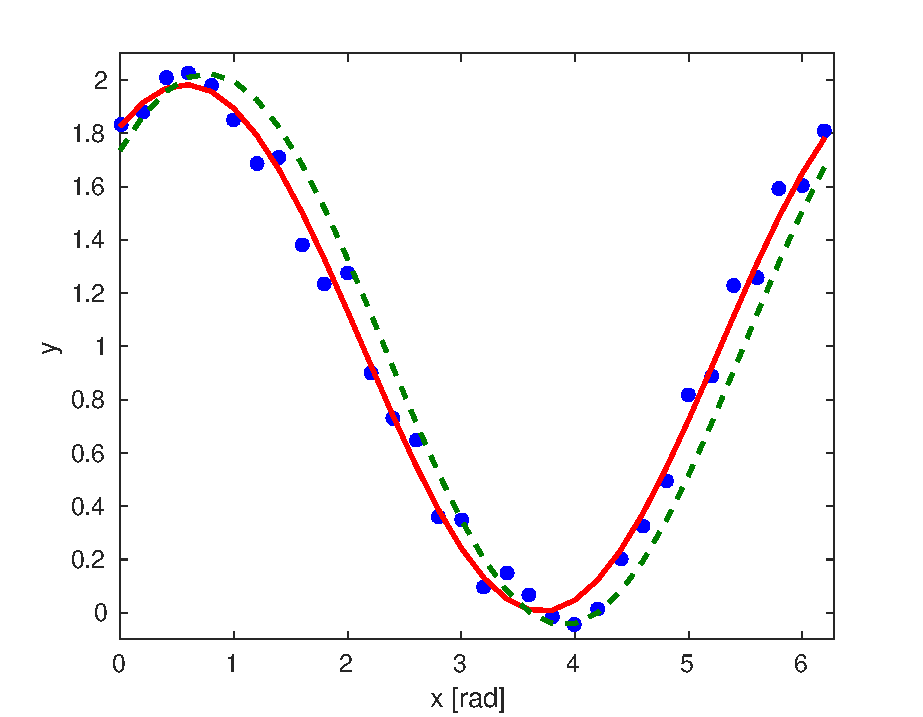
\includegraphics[width=0.9\textwidth]{Figures/phaseMons/sinFitEx}
  \caption{Example sine fit to generated data with added random noise.}
  \label{f:sinFitEx}
\end{figure}

\begin{table}
  \begin{center}
    \begin{tabular}{|c c c c|}
	   \hline
       Parameter & Value & Initial & Fit \\ \hline
       \(A\) & 1 & 1.03 & \(0.99\pm0.02\)\\
       \(b\) & 1 & 1 & \(1.00\pm0.02\) \\
       \(c\) & 1 & 0.81 & \(1.00\pm0.06\) \\
       \(d\) & 1 & 0.99 & \(0.99\pm0.02\) \\ \hline
    \end{tabular}
    \caption{Typical upstream phase and energy conditions at CTF3.}
  	\label{t:sinFitEx}
  \end{center}
\end{table}

\newsection{monSigResponse}{Signal Generator Measurements}

Measurements have been taken using a 12~GHz signal generator to determine the performance of the three sets of phase monitor electronics independently from the phase monitors themselves. In particular, these tests were focused on identifying the saturation and cross-talk characteristics of the output mixer and diode signals in order to determine a suitable input power range to use during normal operation.

\subsection{Experimental Setup}
\label{ss:sigGenSetup}

Two changes were made to the setup shown in Figure~[REF] for these tests. Firstly, the beam induced signal from the phase monitors usually connected to the RF port of the mixers is replaced by the output from a 12~GHz signal generator. To be able to reach the same input power levels as the beam signals the signal generator output is amplified using a [TODO:amplifierInfo]. This allows the input power to the mixers to be varied in a wide range between 0 and 33dBm, or between 0.2 and 10.0~V in terms of voltage. The precise power sent to the mixer is verified between each measurement using a power meter. 

Secondly, the diode outputs were amplified during these tests (using the same amplifier introduced in Section~\ref{ss:sisNoise}) by a factor 10 in voltage to reduce digitiser noise in the measurement. The non-amplified peak diode output is therefore 170~mV, rather than the 1.7~V seen in the plots in this section. The \(\pm500\)~mV mixer outputs have not been amplified. Usually the mixer output is amplified and the diode not amplified, as in Figure~[REF], for reasons that will become clear later in this chapter.

There are some differences between the properties of the generated signal and the beam signal that would be used in normal operation. Firstly, unlike the pulsed beam signal the used generated signal is continuous. It has been verified that the response of the mixers is equivalent for both the continuous and pulsed signals, at least in terms of output power and saturation levels [REF]. The cross-talk properties are difficult to characterise with beam based measurements alone, but assumed to be similar.

Secondly, the phase of the generated signal does not vary with time, compared to the beam signal which has a large \(\sim40^\circ\) phase sag along the pulse and much larger phase jitter. If the signal generator was used at the same frequency as the beam and LO signals, 11.994~GHz, the mixer output would therefore be constant as it depends only on the static phase as per Equation~\ref{e:mixOutSameFreq}. Instead, a generated signal with a slightly lower frequency of 11.991~GHz has been used. From Equation~\ref{e:mixOutAnyFreq} it can be seeen that in this case the mixer output voltage is sinusoidal, with a frequency equal to the frequency difference between the LO and RF inputs -- or \(11.994-11.991\)~GHz = 3~MHz with the setup used here. This has the benefit of being able to see the response of the electronics to all input phases in one measurement, rather than having to take multiple measurements varying the LO phase shifter between each one.

\subsection{Results}
\label{ss:sigGenResults}

Figures~\ref{f:sigGenAllMix1}--\ref{f:sigGenAllDio3} show the mixer and diode outputs for all three sets of electronics at each of the input power levels sent from the signal generator. These will be referred back to and discussed in more detail in the remainder of this section. Some initial observations that are immediately clear from these figures are as follows. All mixer outputs show a sinusoidal oscillation with a frequency of 3~MHz, or 60 samples at the sampling frequency of 192~MHz, as expected. An oscillation with the same frequency is also visible on the diode outputs, with the largest amplitude for the 2nd set of electronics. This is the first hint of the non-ideal characteristics of the diodes. Finally, output of the mixer and diode increases with the input power, as expected. At high input powers the outputs begin to saturate. This is apparent by observing the diode signals, on which the output is much flatter at the highest power levels, without the oscillation seen at low input powers. The characteristics of the mixers are discussed in Section~\ref{ss:sigGenMixer} and the diodes in Section~\ref{ss:sigGenDiode}.

\begin{figure}
  \centering
  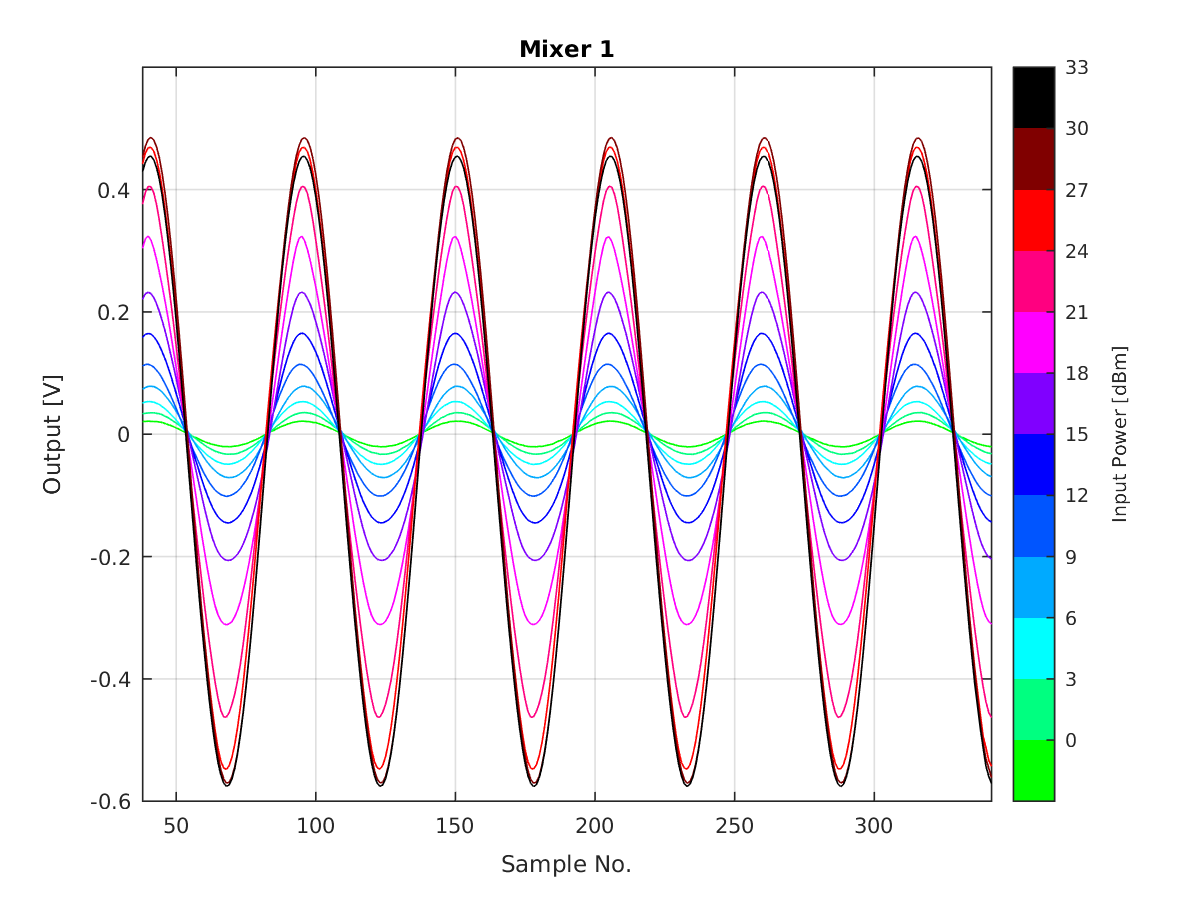
\includegraphics[width=0.9\textwidth]{Figures/phaseMons/Mixer1_AllPowerLevels}
  \caption{Response of Mixer 1 to signal generator input.}
  \label{f:sigGenAllMix1}
  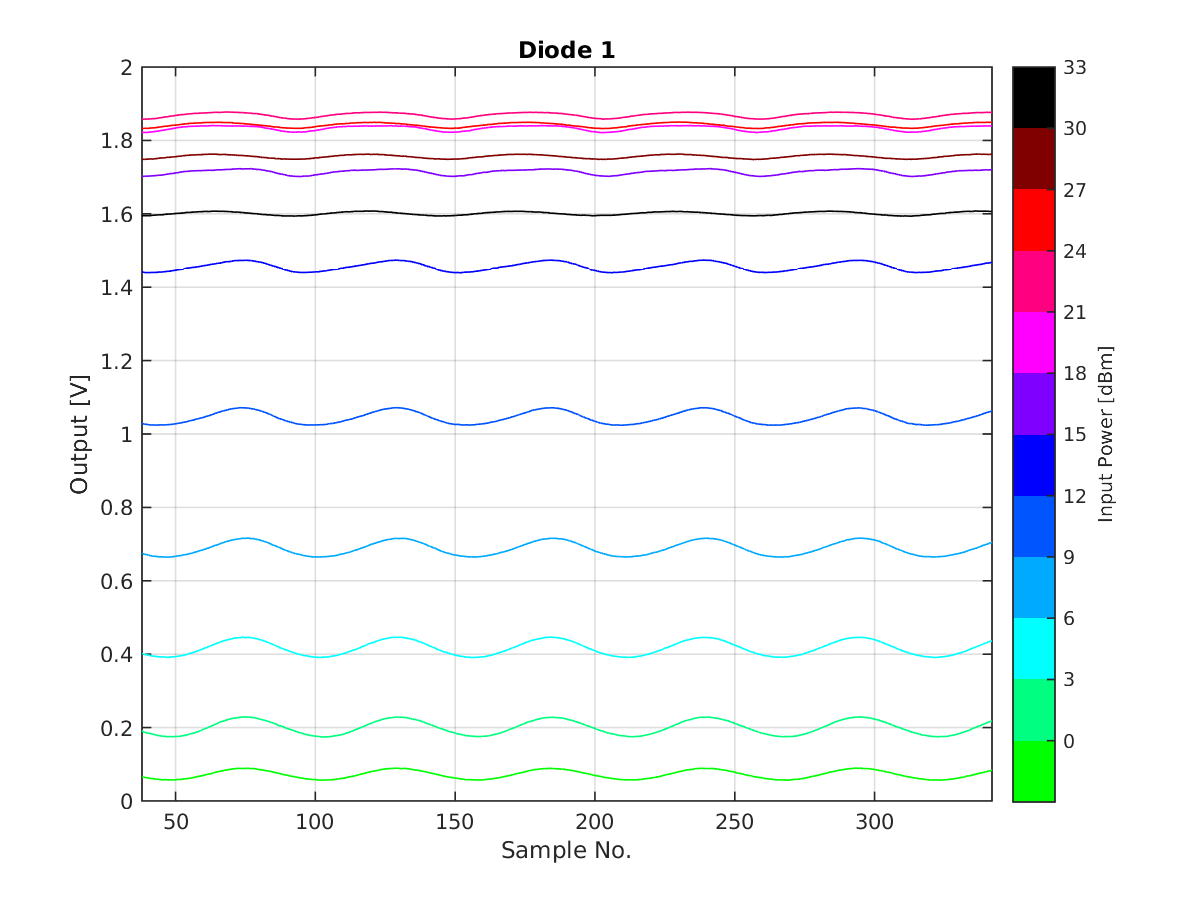
\includegraphics[width=0.9\textwidth]{Figures/phaseMons/Diode1_AllPowerLevels}
  \caption{Response of Diode 1 to signal generator input.}
  \label{f:sigGenAllDio1}
\end{figure}

\begin{figure}
  \centering
  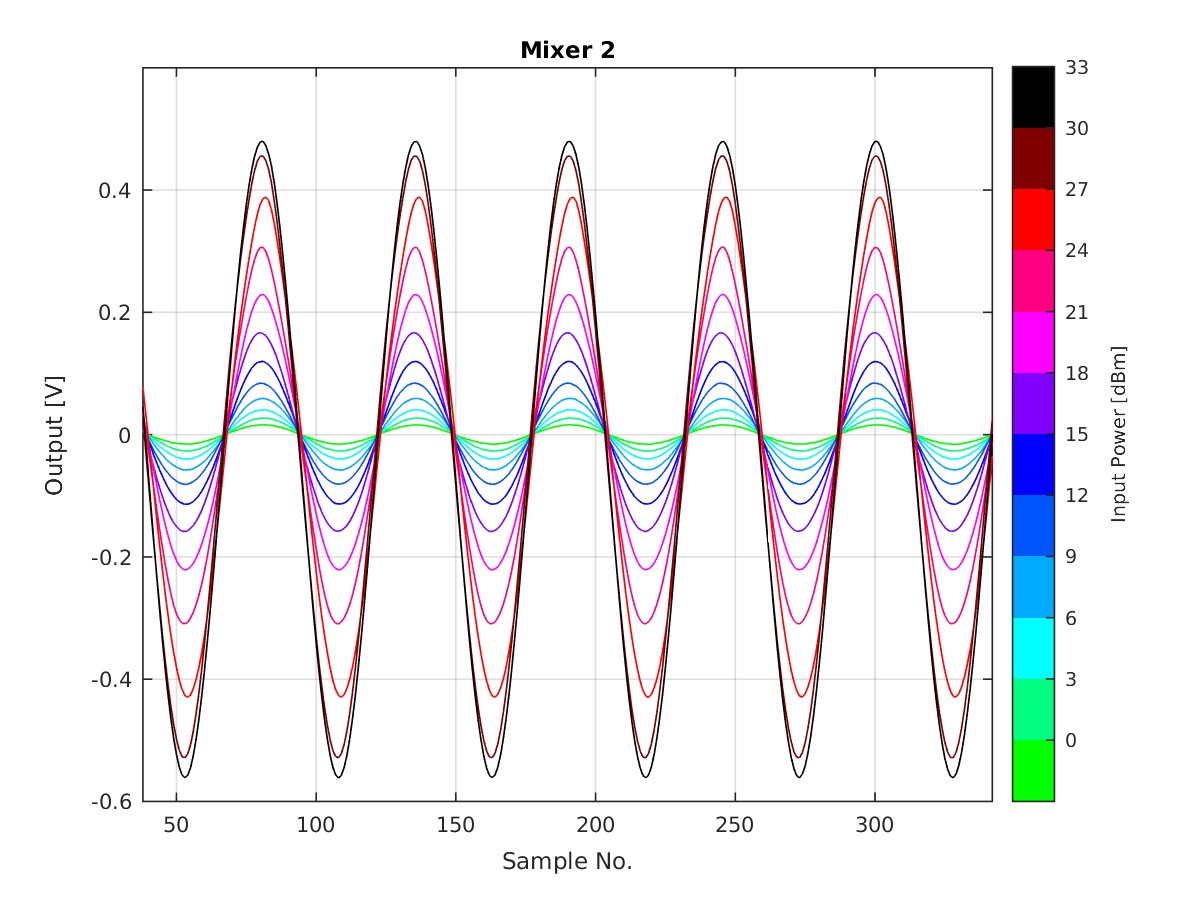
\includegraphics[width=0.9\textwidth]{Figures/phaseMons/Mixer2_AllPowerLevels}
  \caption{Response of Mixer 2 to signal generator input.}
  \label{f:sigGenAllMix2}
  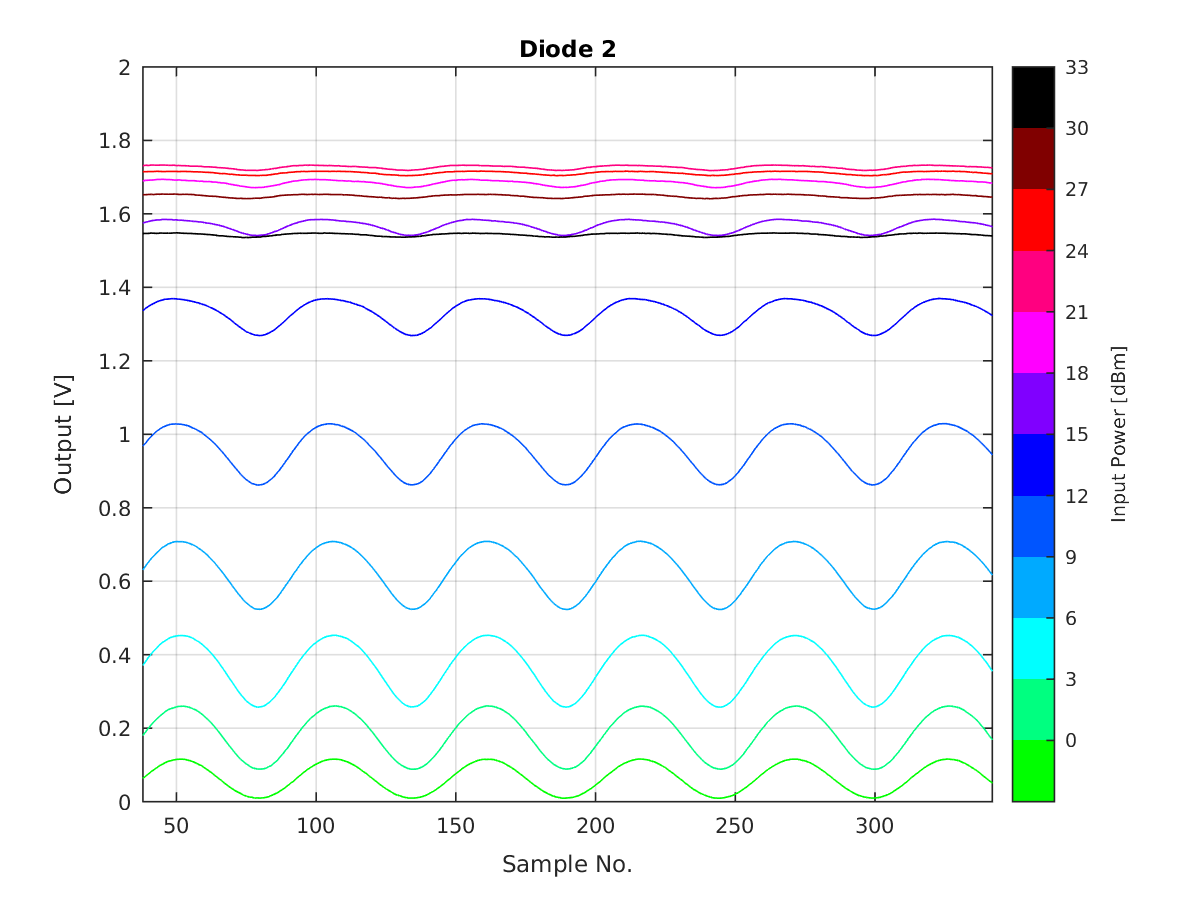
\includegraphics[width=0.9\textwidth]{Figures/phaseMons/Diode2_AllPowerLevels}
  \caption{Response of Diode 2 to signal generator input.}
  \label{f:sigGenAllDio2}
\end{figure}

\begin{figure}
  \centering
  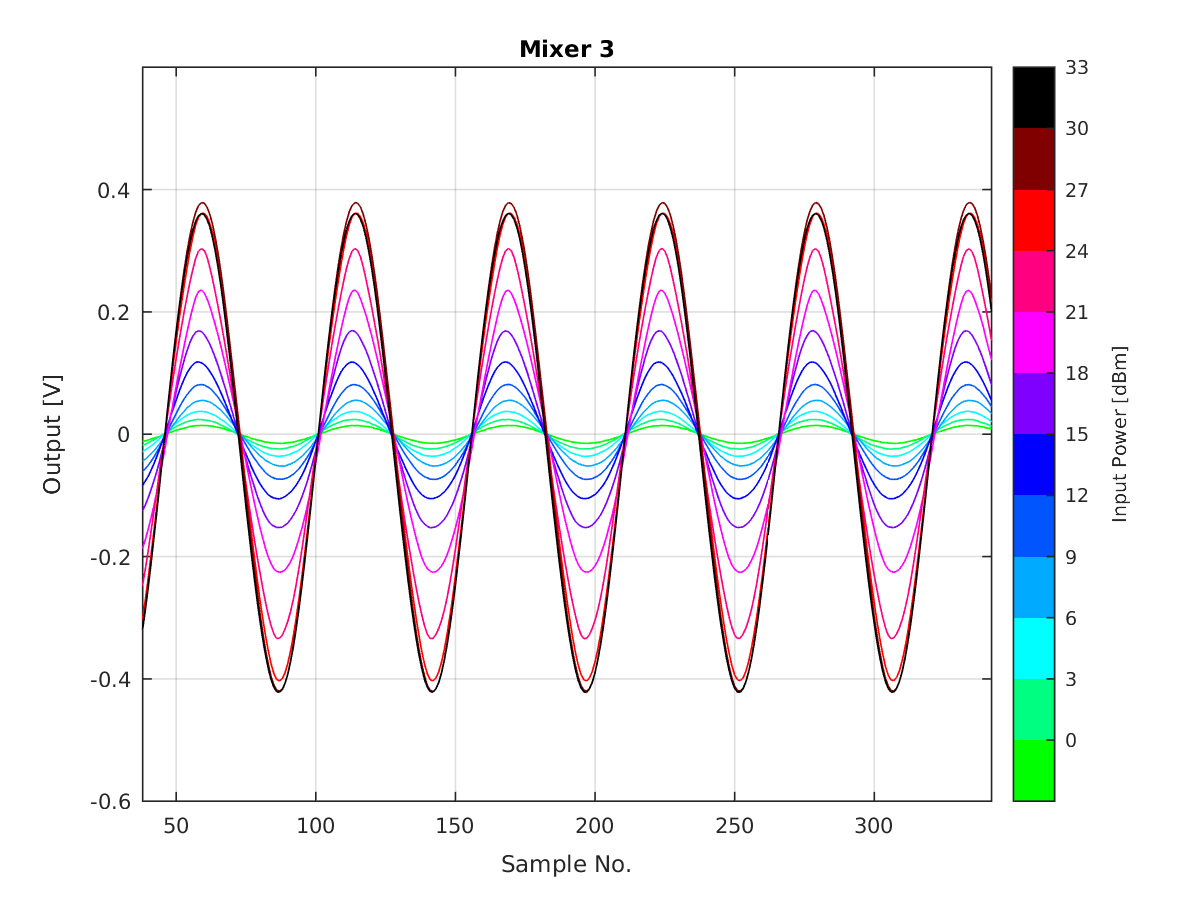
\includegraphics[width=0.9\textwidth]{Figures/phaseMons/Mixer3_AllPowerLevels}
  \caption{Response of Mixer 3 to signal generator input.}
  \label{f:sigGenAllMix3}
  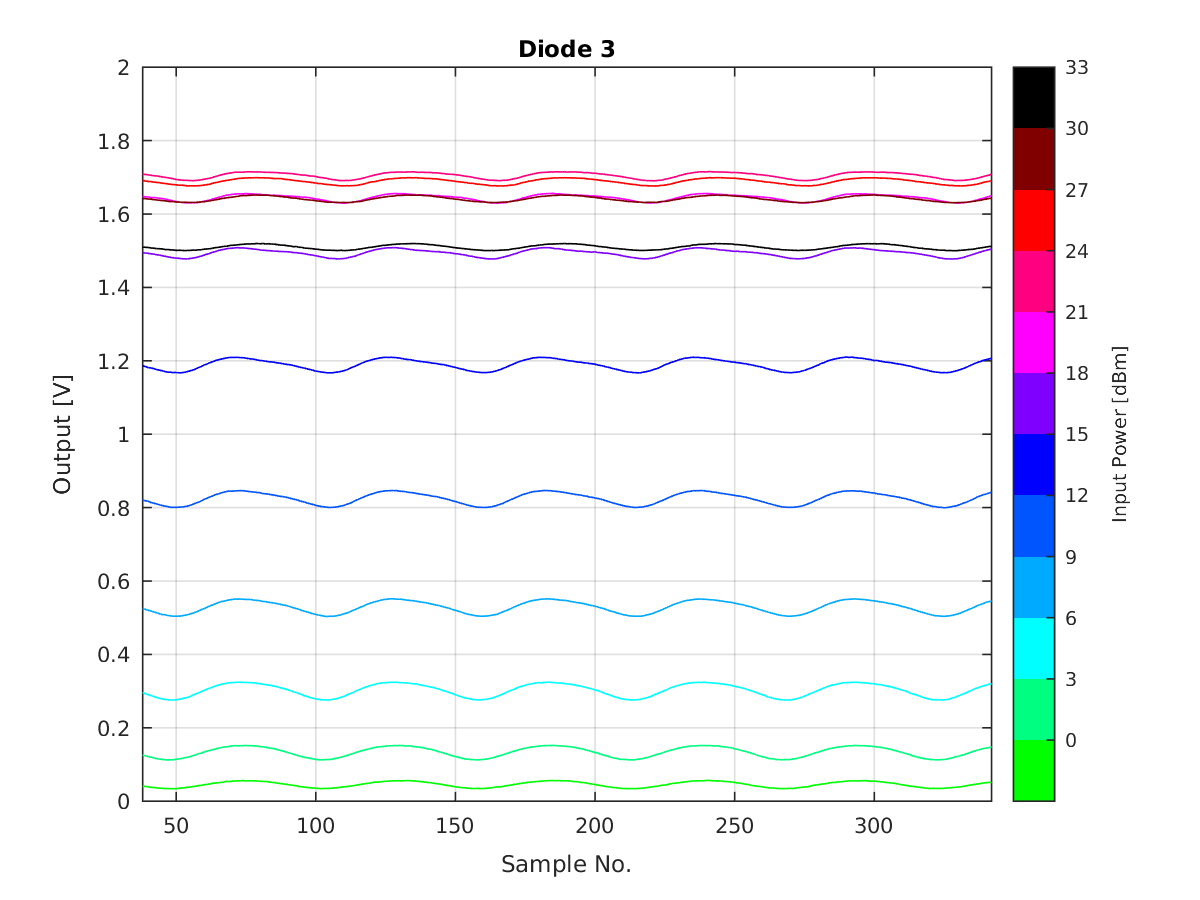
\includegraphics[width=0.9\textwidth]{Figures/phaseMons/Diode3_AllPowerLevels}
  \caption{Response of Diode 3 to signal generator input.}
  \label{f:sigGenAllDio3}
\end{figure}

\subsection{Mixer Performance}
\label{ss:sigGenMixer}

\subsubsection{Sinusoidal Characteristics}

Figure~\ref{f:mixersFit27dBm} shows fits to the response of all mixer outputs at an input power of 27~dBm, close to the typical input power from the beam signals when they are connected. Markers show the data points and the lines are sine fits to the data. The phase offset (displacement in peaks) between the output of each mixer holds no significance for the electronics performance. This is set only by the relative phase between the signal generator and the LO at the time the measurement was started. For normal operation with beam the LO phase shifters are changed to match the phasing of each set of electronics (Section~\ref{s:monCalibrations}).

The reconstruction of the phase from the mixer output depends on the mixer output being sinusoidal. In particular the maximum mixer output, or equivalently the gradient around zero mixer output (using the small angle approximation) is critical due to the dependence on the amplitude in Equation~\ref{e:phaseRecIdeal}. Each set of electronics has a different output amplitude due to slight differences in the LO power for each set of electronics and between the individual components used. At an input power of 27~dBm Mixer 1 has a higher peak output of 510~mV, compared to 410~mV and 380~mV for Mixer 2 and Mixer 3 respectively. 

Overall, the agreement between the actual mixer output and the sinusoidal fits at this input power is good. However, there is some distortion away from the ideal sine curve that is most visible around the maximum and minimum mixer output. Figure~\ref{f:mixersFitResid27dBm} shows the residuals between the mixer outputs and the sine fits across one half wavelength -- from maximum output to minimum output. In the figure the plotted residual is the difference between the fit and the data expressed in terms of an equivalent phase offset, \(\Delta \phi\), using:
\begin{equation}
\Delta \phi(t) = \arcsin\left(\frac{V_{MIXER}(t)-V_{FIT}(t)}{A}\right)
\end{equation}
Where \(V_{MIXER}(t)\) and \(V_{FIT}(t)\) are the mixer voltage and fitted voltage at sample \(t\) respectively, and \(A\) is the fitted mixer amplitude. On the falling slope between the peaks there is only a slight oscillation about the ideal sinusoidal behaviour. The deviation from ideal is at the level of \(0.25\pm0.03^\circ\) and \(0.30\pm0.04^\circ\) for the first and third mixers, with a slightly larger effect of \(0.45\pm0.04^\circ\) for the second mixer. This applies within \(\pm80^\circ\) of the zero crossing in the mixer output. Within \(\pm10^\circ\) of the maximum or minimum output the deviation from the sine fit rapidly increases, reaching several degrees for each mixer. For operation with the beam this means that the accuracy of the phase measurement cannot be guaranteed when the LO phase is set so that the mixer is giving close to its maximum or minimum output. This is also true for other reasons, as seen in Section~\ref{s:resolution}. The PFF system can only correct small offsets at the level of around \(\pm5^\circ\) (Section~\ref{ss:corrRange}), so the non-ideal response close to peak output is not an issue for the PFF performance.

\begin{figure}
  \centering
  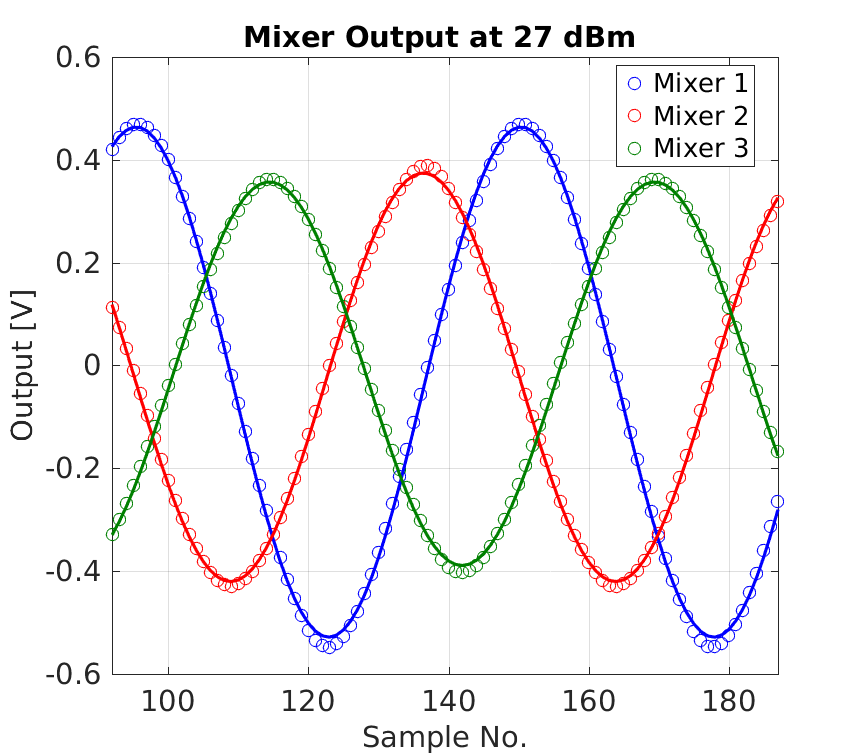
\includegraphics[width=0.9\textwidth]{Figures/phaseMons/mixersFit27dBm}
  \caption{Sinusoidal fit to mixer responses at 27~dBm input power.}
  \label{f:mixersFit27dBm}
\end{figure}

\begin{figure}
  \centering
  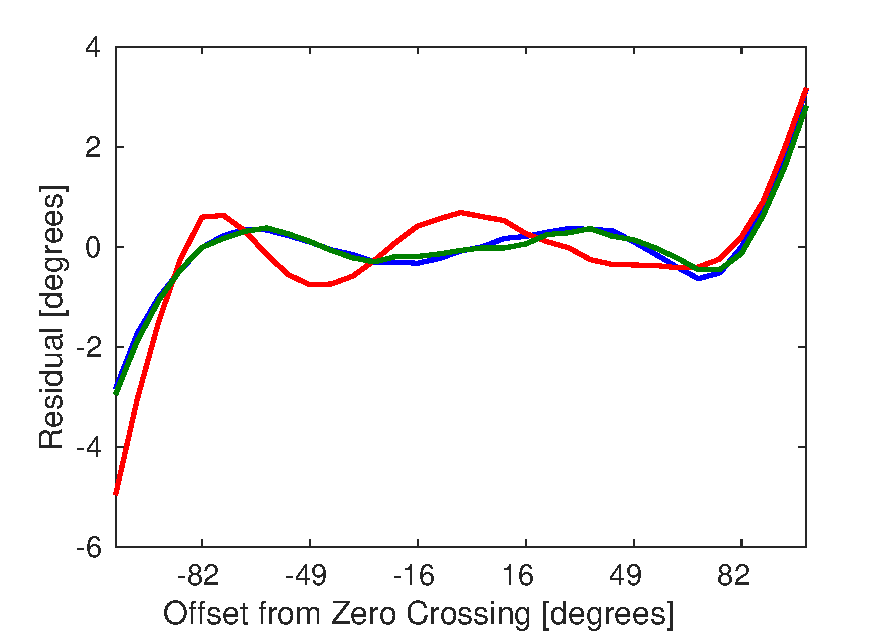
\includegraphics[width=0.9\textwidth]{Figures/phaseMons/mixersFitResid27dBm}
  \caption{Residuals to sinusoidal fit at 27dBm.[TODO: sample numbers don't relate to previous plots]}
  \label{f:mixersFitResid27dBm}
\end{figure}

However, for input powers in the range from 15--21~dBm the non-ideal characteristics of the mixers are larger. One example of this is shown in Figure~\ref{f:mixersFit18dBm}, at an input power of 18~dBm. If input powers in this range are used calibrations of the mixer response should normally be restricted to around the zero crossing so that the fitted amplitude gives the best approximation to the true behaviour for small phase offsets. 

\begin{figure}
  \centering
  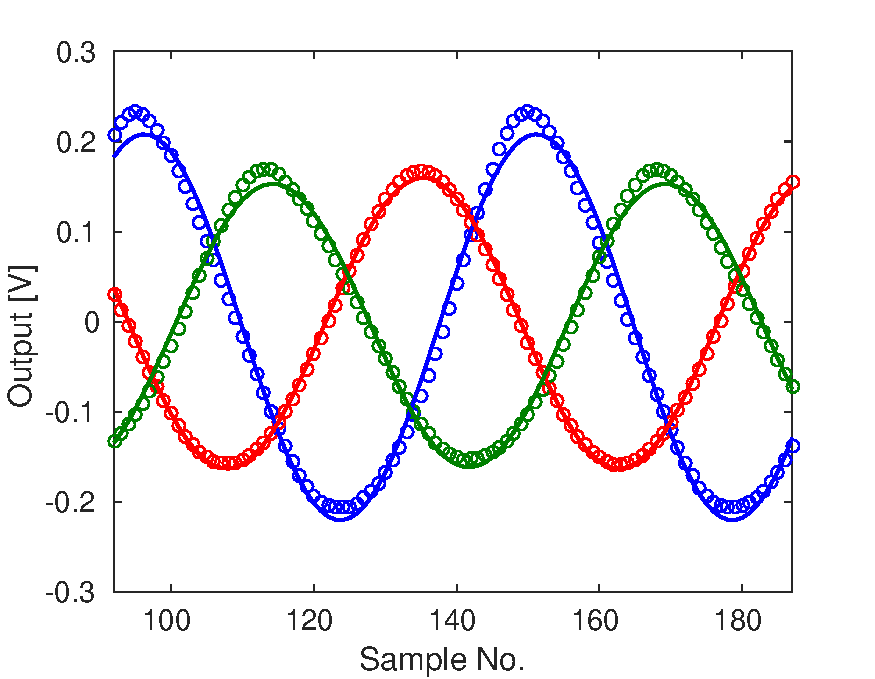
\includegraphics[width=0.9\textwidth]{Figures/phaseMons/mixersFit18dBm}
  \caption{Sinusoidal fit to mixer responses at 18~dBm input power.}
  \label{f:mixersFit18dBm}
\end{figure}

\subsubsection{Dependence on Input Power}

The mixer output is expected to linearly depend on the input voltage and the diode on the square of the input voltage. Both these dependencies must hold in order to use Equation~\ref{e:phaseRecIdeal} and obtain a phase measurement that does not depend on the input voltage to the electronics (therefore making the calculated phase insensitive to any possible variations in power along the pulse from the beam signal, for example). For these measurements the input voltage can be calculated using the known input power and 50~\(\Omega\) impedance of the electronics.

Figure~\ref{f:LinFitMixerVsVolts} shows the dependence of the mixer output amplitudes on the input voltage. As seen previously the first mixer gives a larger output than the other two mixers. The 2nd and 3rd mixers give a similar response up to an input voltage of 3.5~V (24~dBm). Dashed lines in the figure show a linear fit to the mixer output restricted to the range between 0.45~V and 1.75~V (6~dBm to 18~dBm) in each case, as marked by the vertical black lines. All three mixers give a linear response up to an input voltage of around 3~V (23~dBm), after which the effects of saturation begin to appear. By an input voltage of 5~V (27~dBm) the first and third mixers are almost fully saturated with almost no remaining power dependence in the output. The second mixer begins to enter saturation at the same voltage as the other two mixers but retains a strong power dependence up to a higher input voltage of 7~V (30~dBm).

\begin{figure}
  \centering
  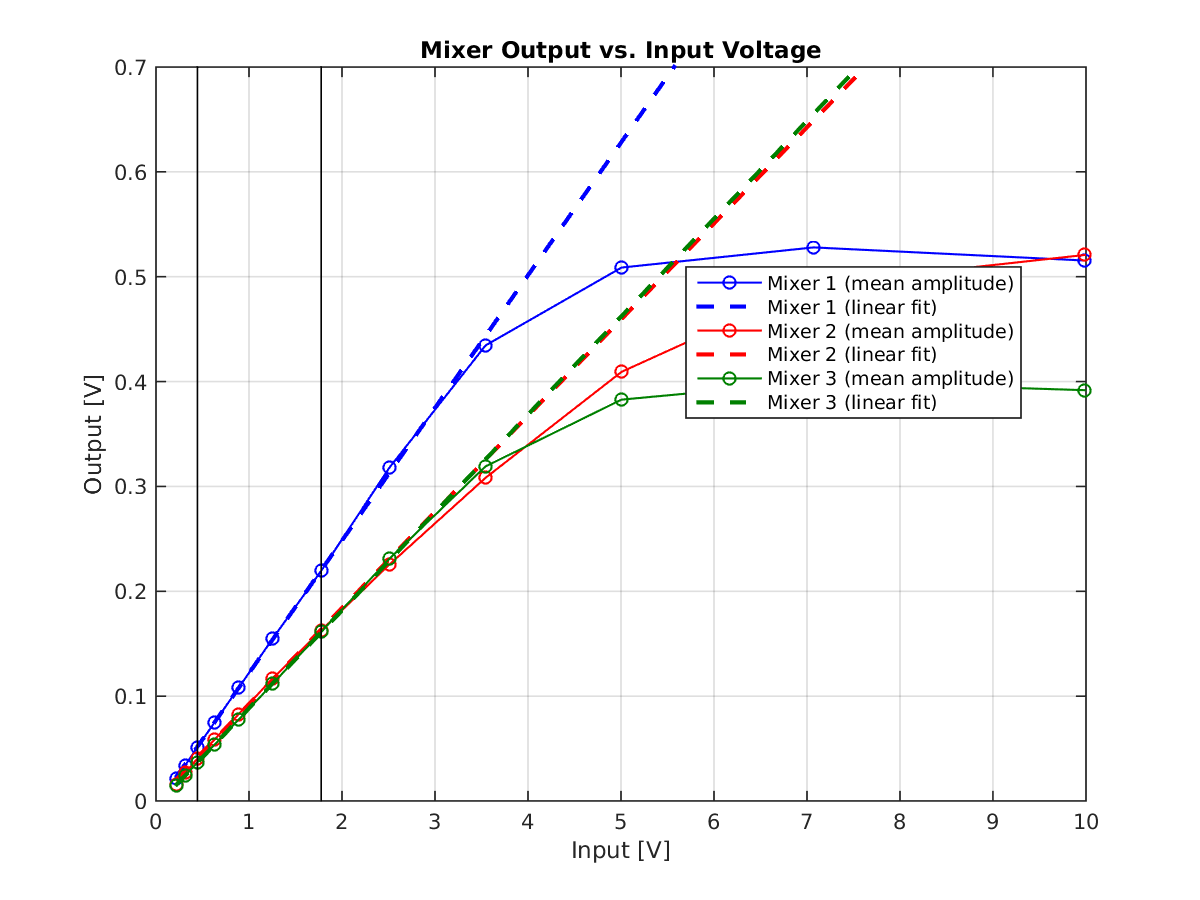
\includegraphics[width=0.9\textwidth]{Figures/phaseMons/LinFitMixerVsVolts}
  \caption{Linear fit to mixer output voltage vs. input voltage.}
  \label{f:LinFitMixerVsVolts}
\end{figure}


\subsubsection{Asymmetry in Output}

One final interesting property of the mixers is that the output is not symmetric about zero, in other words the maximum output voltage is different to the absolute value of the minimum output voltage. This is perhaps most visible looking back to the Mixer~1 output at all power levels in Figure~\ref{f:sigGenAllMix1}, where the maximum output is around \(+0.45~V\) but the minimum output is around \(-0.55~V\).

Figure~\ref{f:MixerVsVolts} shows how the mixer amplitude at maximum and minimum output varies with the input voltage. Mixer~1 asymmetry is largest for Mixer~1 and smallest for Mixer~3. The effect appears to increase in magnitude with the input voltage, with the \(\sim100\)~mV difference mentioned previously for Mixer~1 at an input of 10~V, but differences of only several mV at low input powers. For each mixer the amplitude at maximum output is larger for input voltages up to 2.5~V (21~dBm). Above 2.5~V input voltage this flips, with the minimum mixer amplitude being larger than the maximum amplitude.

\begin{figure}
  \centering
  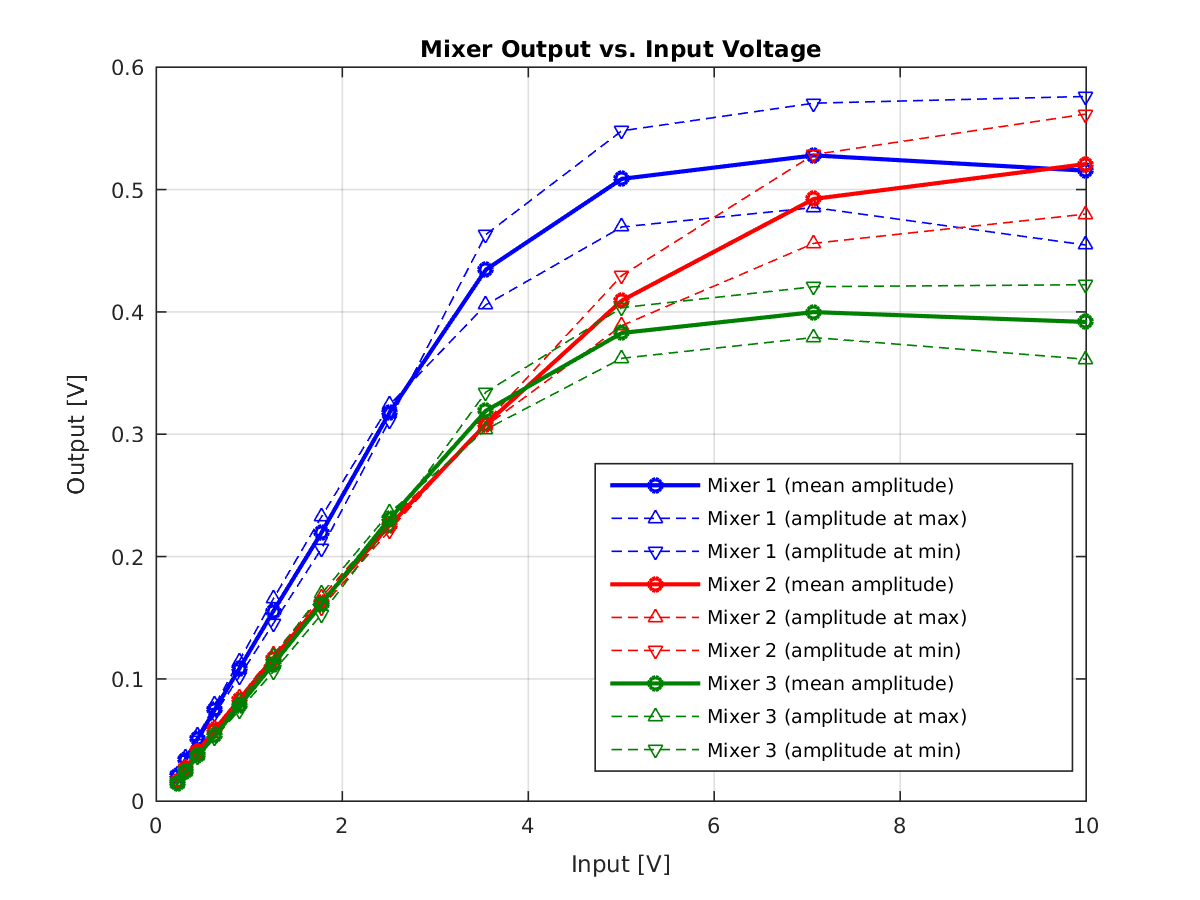
\includegraphics[width=0.9\textwidth]{Figures/phaseMons/MixerVsVolts}
  \caption{Mixer output voltage vs. input voltage.}
  \label{f:MixerVsVolts}
\end{figure}

For input voltages between 0.45~V and 1.25~V (6~dBm to 15~dBm) the mixer asymmetry has an approximate quadratic dependence on the input voltage, as shown in Figure~\ref{f:MixerAsymmetryVsVolts}. Outside this range there is no simple relationship that can explain the dependence of the asymmetry on the input voltage. One explanation for the asymmetry in the mixer outputs is cross-talk coming from the diode signals. Above 15~dBm the diodes enter saturation, as discussed in the next section, which may explain why the quadratic fit to the mixer asymmetry is only valid at power levels up to this value. 

\begin{figure}
  \centering
  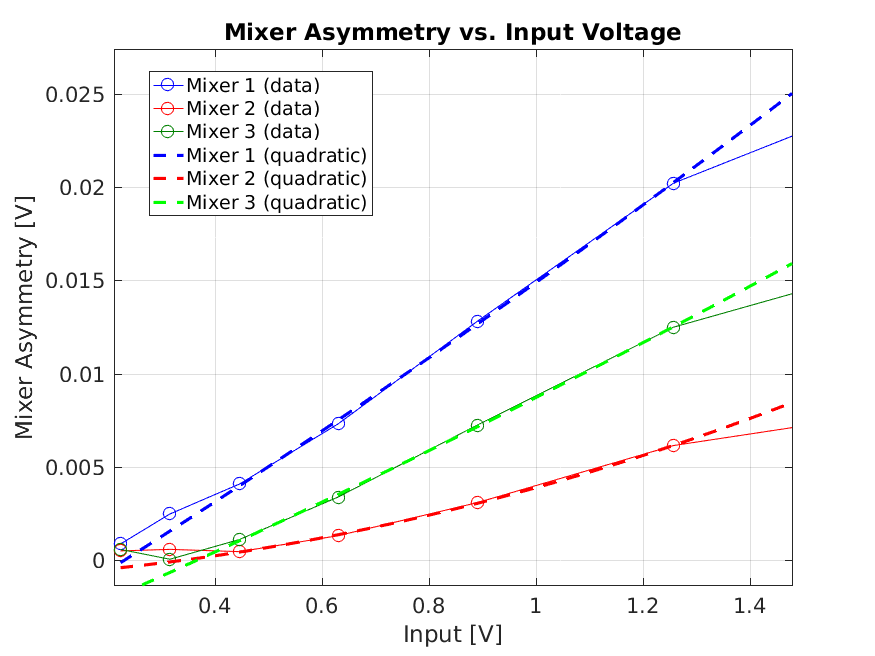
\includegraphics[width=0.9\textwidth]{Figures/phaseMons/MixerAsymmetryVsVolts}
  \caption{Relative amplitude vs. input power of cross-talk on the mixer from the diode.}
  \label{f:MixerAsymmetryVsVolts}
\end{figure}

Taking the power dependent asymmetry in to account the actual mixer response can be modified from Equation~\ref{e:mixOutSameFreq} to become:
\begin{equation}
\mathrm{Mixer}(t) = m_1A(t)\sin[\phi(t)] + m_2A(t)^2 + m_3A(t) + m_4
\label{e:actualMixerResponse}
\end{equation}
Where \(A(t)\) is the input voltage at time \(t\), and \(m_1\), \(m_2\), \(m_3\), and \(m_4\) are calibration constants.

\subsection{Diode Performance}
\label{ss:sigGenDiode}

\subsubsection{Dependence on Input Power}

The dependence of the three diode outputs on the input power is shown in Figure~\ref{f:SqrtDiodeVsVolts}, with the square root of the diode output plotted rather than the diode directly as this is the expected linear relationship. Immediately it is apparent that the diode signals saturate at much lower input voltages than the mixer signals. All three diodes are almost fully saturated at an input of 2~V (20~dBm), with the effects of saturation already beginning to appear above 1.25~V (15~dBm). Figure~\ref{f:LinFitSqrtDiodeVsVolts} shows a linear fit to the square root of the diode, using the range of input voltages between 0.45~V and 1.25~V (6--15~dBm). Even below saturation the response of sqrt(Diode) is not well approximated by a linear dependence as desired. However, in the range from 0.30~V 1.25~V (3~dBm to 15~dBm) a quadratic fit to the diode output directly (not sqrt(Diode)) does give a good approximation to the true dependence of the diodes on the input voltage. This is shown in Figure~\ref{f:QuadFitDiodeVsVolts}.

\begin{figure}
  \centering
  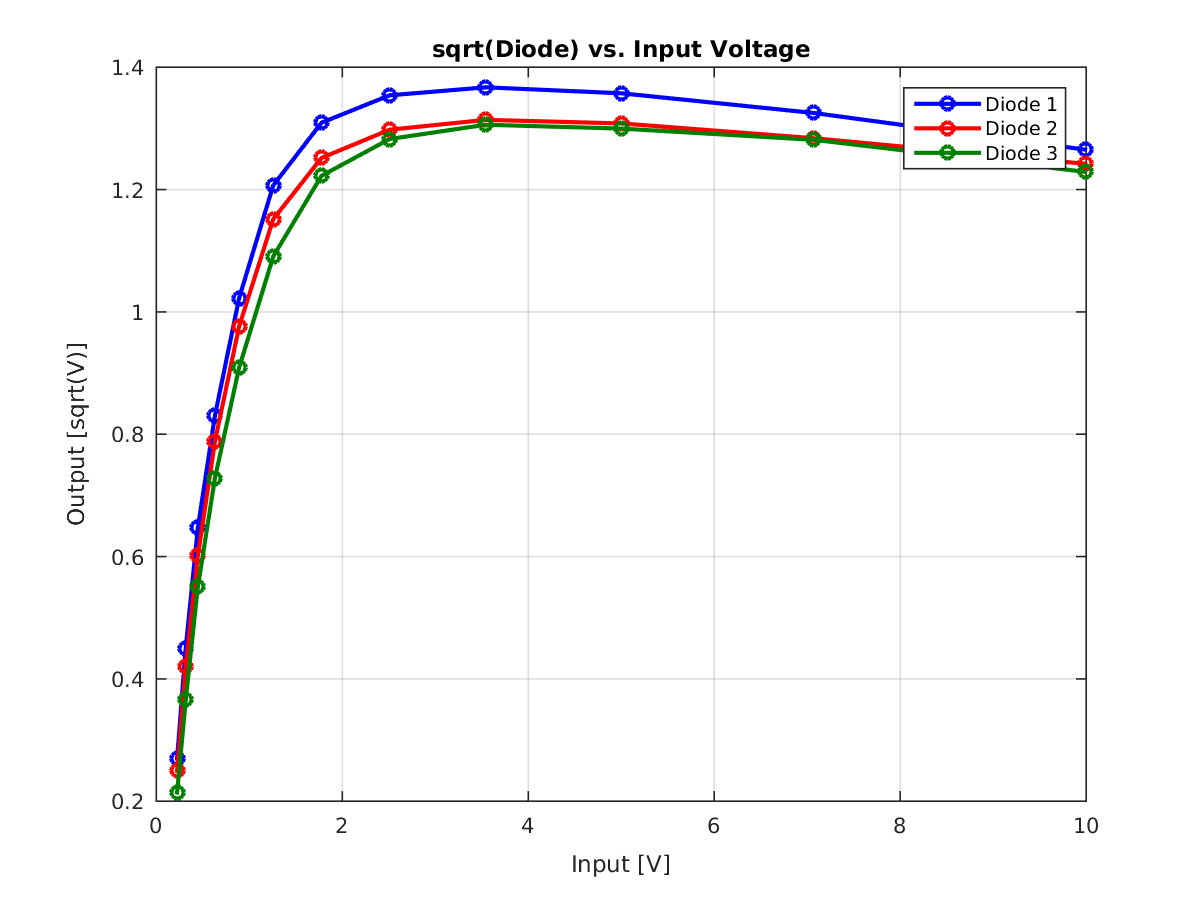
\includegraphics[width=0.9\textwidth]{Figures/phaseMons/SqrtDiodeVsVolts}
  \caption{sqrt(Diode) vs. input voltage.}
  \label{f:SqrtDiodeVsVolts}
\end{figure}

\begin{figure}
  \centering
  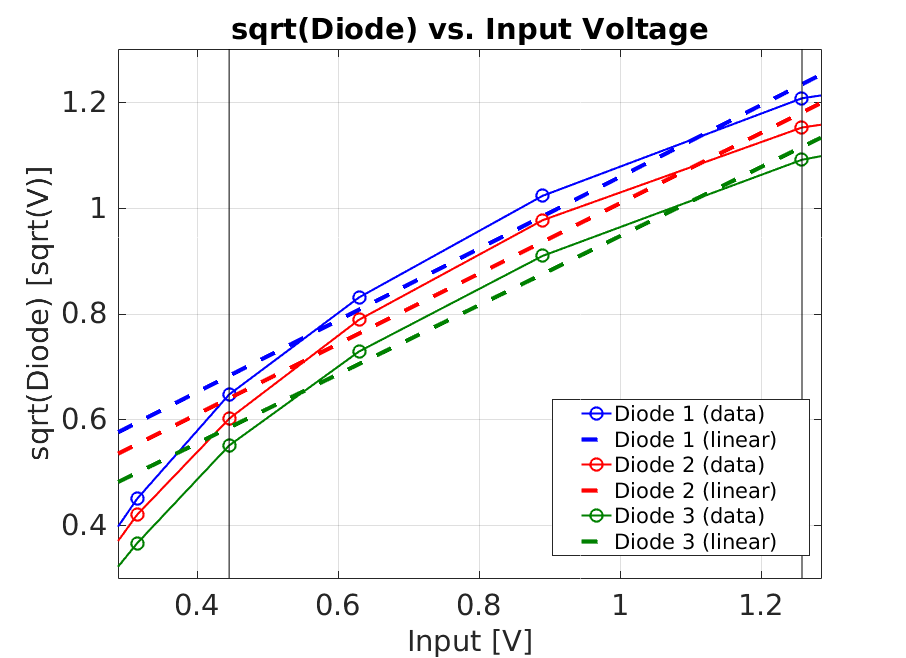
\includegraphics[width=0.9\textwidth]{Figures/phaseMons/LinFitSqrtDiodeVsVolts}
  \caption{Linear fits to sqrt(Diode) vs. input voltage.}
  \label{f:LinFitSqrtDiodeVsVolts}
  \centering
  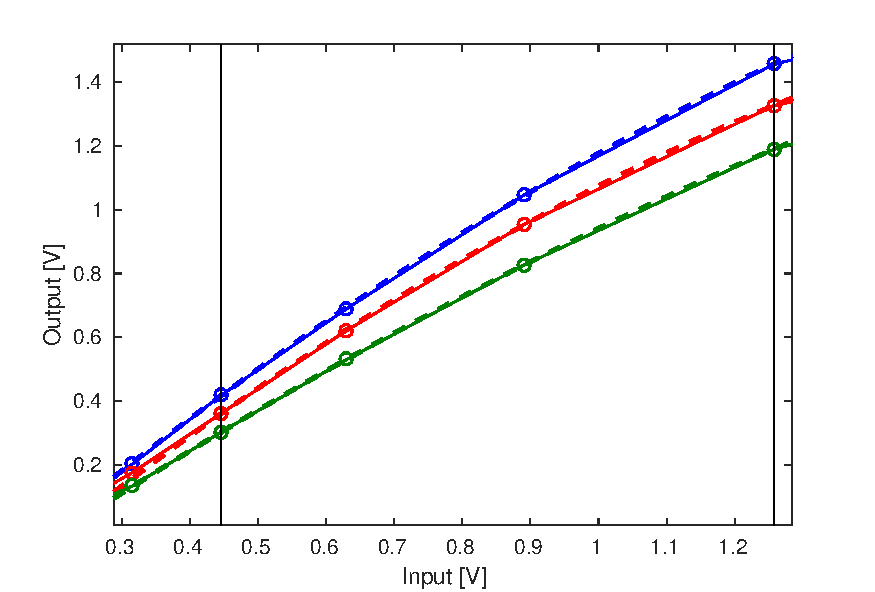
\includegraphics[width=0.9\textwidth]{Figures/phaseMons/QuadFitDiodeVsVolts}
  \caption{Quadratic fits to Diode vs. input voltage.}
  \label{f:QuadFitDiodeVsVolts}
\end{figure}

\subsubsection{Cross-Talk}

As seen previously in Figures~\ref{f:sigGenAllDio1},~\ref{f:sigGenAllDio2}~and~\ref{f:sigGenAllDio3} the diode outputs show a sinusoidal oscillation. Like there is cross-talk from the diode on the mixer outputs, there is also cross-talk from the mixers on the diode outputs. Figure~\ref{f:Diode1_Power6} shows a sinusoidal fit to the cross-talk on Diode~1 at an input power of 6~dBm. It has the same characteristics as the mixer output, including the slight distortion away from ideal sinusoidal behaviour around the peaks. However, as the diodes enter saturation the oscillation is initially distorted, and then has a much smaller amplitude when the diode output is fully saturated. One example of this is shown for the Diode~1 output at 18~dBm in Figure~\ref{f:Diode1_Power18}. The peaks around the maximum output are clearly non-sinusoidal in this case.

\begin{figure}
  \centering
  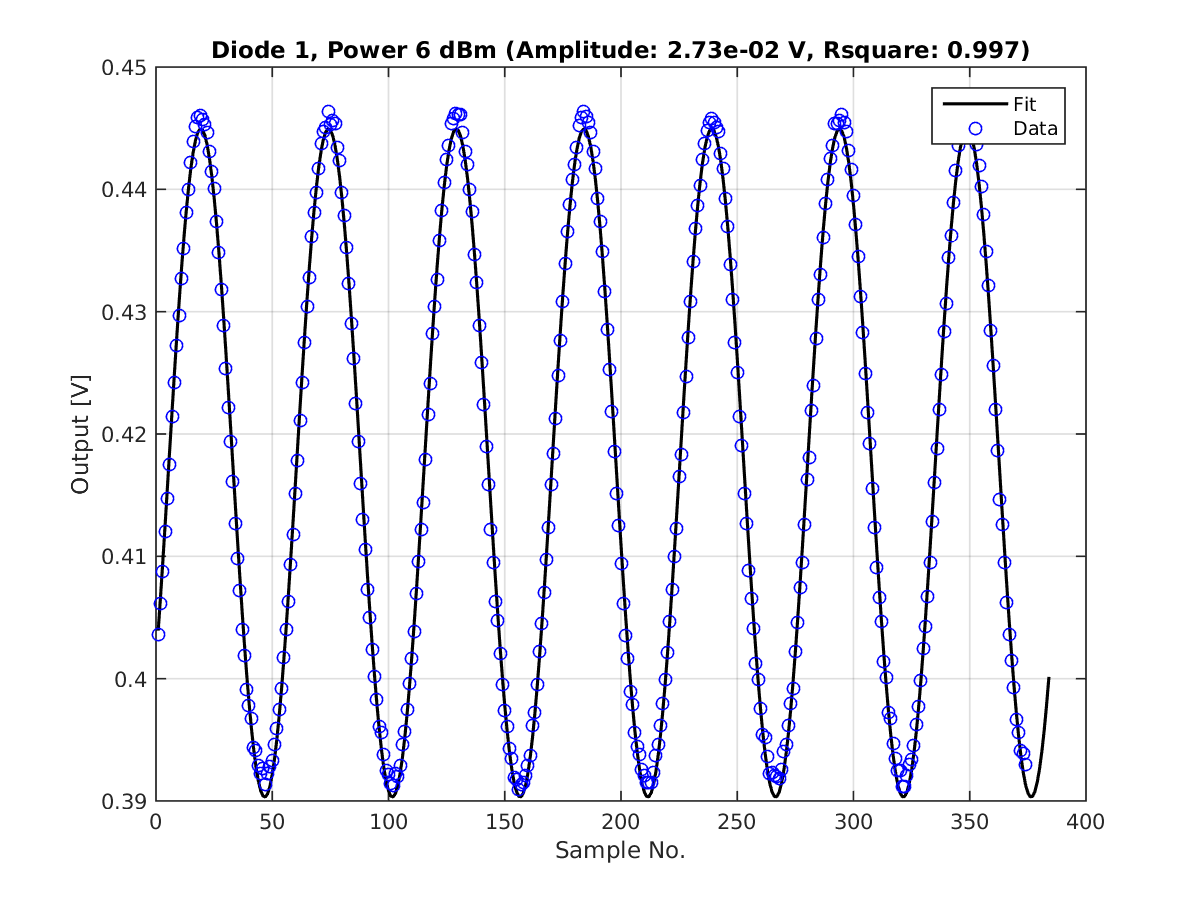
\includegraphics[width=0.9\textwidth]{Figures/phaseMons/Diode1_Power6}
  \caption{Sinusoidal fit to cross-talk on diode at 6~dBm input power.}
  \label{f:Diode1_Power6}
\end{figure}

\begin{figure}
  \centering
  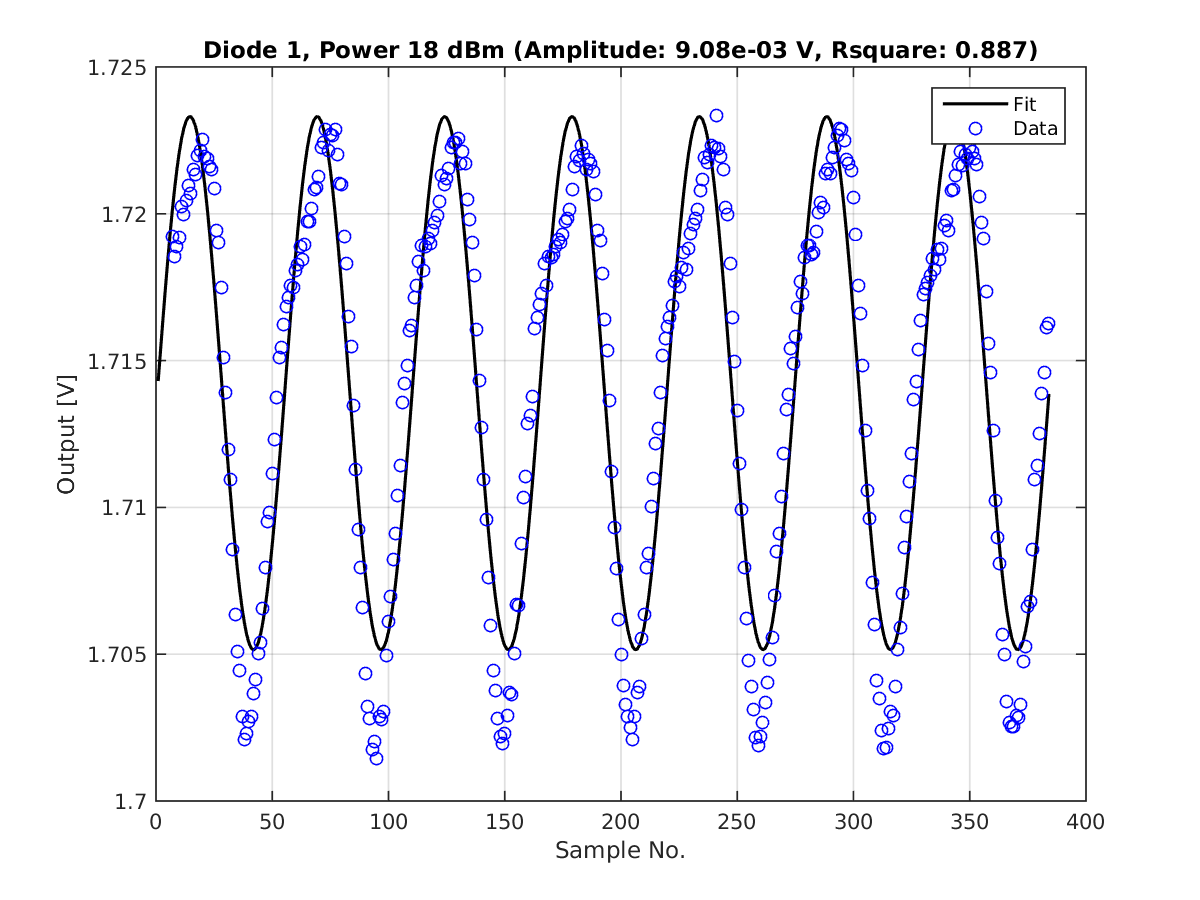
\includegraphics[width=0.9\textwidth]{Figures/phaseMons/Diode1_Power18}
  \caption{Sinusoidal fit to cross-talk on diode at 18~dBm input power.}
  \label{f:Diode1_Power18}
\end{figure}

Figure~\ref{f:RelativeDiodeXTalkVsPower} shows the dependence of the relative amplitude of the cross-talk on the input power. The relative amplitude of the cross-talk means the fitted amplitude of the sinusoidal oscillation on the diode divided by the mean diode output. Up until the diode outputs are fully saturated the relative amplitude of the cross-talk is around a factor two larger for the second diode. For example, at an input power of 12~dBm the relative cross-talk is at around the level of 30\% for the second diode, or 15\% for the first and third diode outputs. Up to input powers of 15~dBm the relative cross-talk is always above 10\%.

\begin{figure}
  \centering
  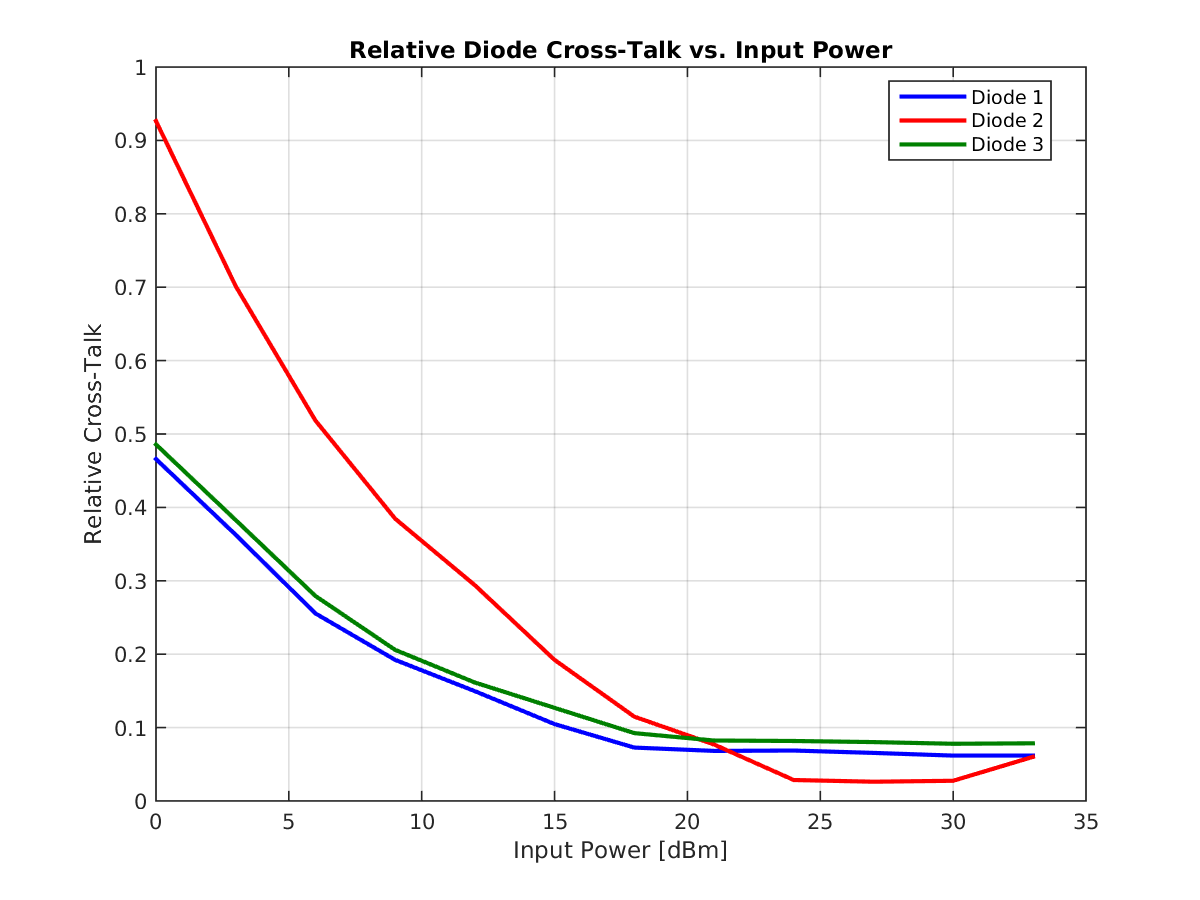
\includegraphics[width=0.9\textwidth]{Figures/phaseMons/RelativeDiodeXTalkVsPower}
  \caption{Dependence of the relative amplitude of cross-talk on the diode versus the input power.}
  \label{f:RelativeDiodeXTalkVsPower}
\end{figure}

Finally, Figure~\ref{f:PhaseDiodeVsMixer} compares the oscillation on the diode to the oscillation on the mixer. It can be seen that there is a phase shift between the two, which adds a further complication to the necessary phase reconstruction method. Taking in to account the actual characteristics of the diodes, including the cross-talk and quadratic dependence on the input power, the expected expression for the diode output from Equation~\ref{e:idealDiode} can be modified to:
\begin{equation}
\mathrm{Diode(t)} = d_1A(t)^2 + d_2A + d_3 + d_4A(t)\sin[\phi(t)+\delta]
\label{e:actualDiodeResponse}
\end{equation}
Where \(d_1\), \(d_2\), \(d_3\), \(d_4\) and \(\delta\) are calibration constants.

\begin{figure}
  \centering
  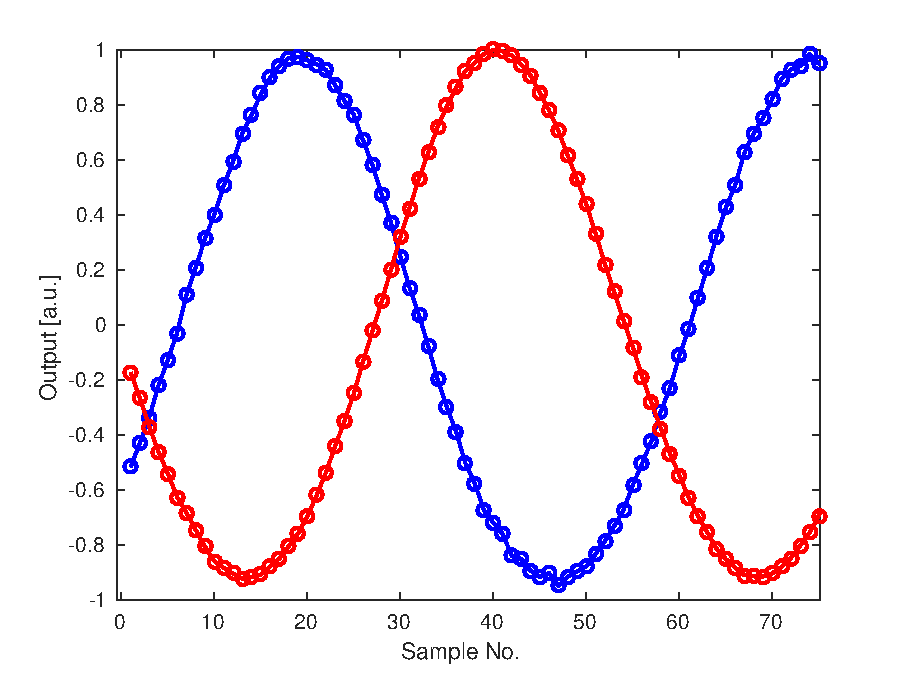
\includegraphics[width=0.9\textwidth]{Figures/phaseMons/PhaseDiodeVsMixer}
  \caption{Comparison of the oscillation on the mixer and the diode, showing a relative phase offset between the two.}
  \label{f:PhaseDiodeVsMixer}
\end{figure}

\subsection{Consequences for Normal Operation}
\label{ss:sigGenConsq}

The results of the signal generator tests have several consequences for the setup of the electronics and phase reconstruction during normal operation with the beam induced signals from the phase monitors. Firstly, in order to maximise the signal to noise ratio and yield the best possible resolution on the phase measurement the highest possible input power below saturation should normally be used. The degradation of the phase resolution with the input power is seen for beam based measurements in Section~[REF]. However, the diodes begin to enter saturation much earlier than the mixers, at around 15~dBm rather than 23~dBm. This means that in order to be able to use the diode measurement as part of the phase reconstruction the input power would have to be limited to below 15~dBm, 8~dBm lower than would be ideal for the mixer performance. There is no way to use different input powers for the mixers and diodes without a complete redesign of the electronics.

Secondly, the modifications that the cross-talk on the mixer and diode make to Equations~\ref{e:actualMixerResponse}~and~\ref{e:actualDiodeResponse} above makes the needed calculation to reconstruct the phase much more complex than the ideal case using Mixer/sqrt(Diode) in Equation~\ref{e:phaseRecIdeal}. In particular, the dependence of the diode output on \(\sin(\phi+\delta)\) means there is no simple expression that can be derived to create an input power independent phase measurement. An iterative process would have to be used to estimate the phase instead, converging towards the true diode output without cross-talk after each iteration using the estimated phase value. This may be possible in offline data analysis but would be difficult to implement in the PFF algorithm whilst still meeting latency requirements.

Due to these reasons, and with no possibility to make modifications to the electronics, the decision was eventually taken to not include the diode measurement in the phase reconstruction process. For operation with the beam this means making the assumption that the output power from the phase monitors is constant along the pulse, and that the jitter in the output power is small. This is a good approximation, as seen later in Section~[REF]. To reduce the sensitivity to any slow drifts in the output power due to changes in the beam conditions calibrations are taken at regular intervals between measurements.

With this treatment of the electronics outputs the phase is reconstructed as follows:
\begin{align}
&\mathrm{Mixer}(t) = A\sin[\phi(t)] + d \\
&\phi(t) = \arcsin\left(\frac{\mathrm{Mixer}(t)-d}{A}\right)
\label{e:phaseRecUsed}
\end{align}
Two calibration constants are needed -- \(A\) and \(d\). \(A\) is the fitted amplitude of the sinusoidal mixer output, and \(d\) is the asymmetry or offset between the maximum and minimum mixer output. This is a simplified form of Equation~\ref{e:actualMixerResponse} given the assumption that the power is constant. In reality both \(A\) and \(d\) have a power dependence.

As any variations in input power are not removed by this method there is a benefit to operating the mixer in a region where the power dependence of the output is reduced. The best phase resolution achieved to date has been achieved with input powers to the electronics in the range between 24.5~dBm and 27~dBm (as stated in [REF]), where the mixers have actually begun to enter saturation, as a result. Operating in this range also has the benefit of reducing the deviation from ideal sinusoidal behaviour at lower input powers as seen in Section~\ref{ss:sigGenMixer}.

All the beam based measurements in the remainder of this chapter and the rest of the thesis use this phase reconstruction approach. Although the diodes are no longer directly used as part of the phase measurement they are still useful for the purposes of the time alignment of signals and for monitoring whether there have been any large changes in input power. The PFF firmware on the FONT5a feedforward controller has also been changed to add the option to not include the diode in the correction calculation (Section~\ref{ss:fontDAQ}). The nominal PFF setup, as used for the results presented in Chapter~\ref{c:feedforward}, now does not use diode normalisation.

\newsection{monCalibrations}{Calibrations}

The remainder of this chapter presents the performance of the complete phase monitor and electronics system for normal operation with the beam, replacing the signal generator with the RF output from the phase monitors. 

The first step in using the the phase monitor measurements is to calibrate the mixer outputs. Calibrations of the phase monitor signals are typically taken on a daily basis during data taking periods, as well as additional calibrations when there have been any changes in beam conditions or to the setup of the electronics. These are needed to determine the calibration constants, amplitude and offset, to be able to determine the phase from the mixer output as previously discussed. This section presents typical calibration results for all three phase monitors and discusses aspects such as the stability of the calibration along the pulse and determining the optimal set point for the LO phase shifters. 

For beam based measurements calibrations are performed using the LO phase shifters. By varying the LO phase shifter the phase between the LO and the beam signal is changed. During a calibration the phase shifters are moved through \(360^\circ\) at 12~GHz  so that the response of the mixer to all phase offsets between the beam and LO can be determined. Normally calibrations are taken at 12 shifter settings across the full \(360^\circ\) range, with 10 pulses acquired at each setting and the whole scan taking approximately 10~minutes. These choices are a compromise between having enough points for a good quality fit whilst reducing the possibility of large drifts in beam phase during the scan which would degrade the fit results. All the calibrations presented use the electronics setup with the mechanical LO phase shifters in place (Section~\ref{s:shifters}). The settings on these phase shifters approximately correspond to degrees at 4~GHz, thus a phase shifter change of 120 units corresponds to \(360^\circ\) at 12~GHz.

A calibration from both the SiS digitiser and FONT5a setup will be shown. During operation of the PFF system Mon~1 is usually connected to the FONT5a board as the correction input, whilst Mon~2 and Mon~3 are connected to the SiS digitisers where they can be acquired together with other signals at CTF3. The difference in measured output voltage between the two setups results from the use of an amplifier before the SiS digitisers to reduce noise in that setup (Section~\ref{s:monDigitisers}). Also, when using the FONT5a board the mixer outputs are attenuated by 1~dB to avoid saturating the FONT ADCs. The calibration constants from Mon~1 on the FONT5a board are needed for the PFF gain calculation in Section~\ref{ss:pffFirmware}. All measurements of the upstream and downstream phase after this chapter use Mon~2 and Mon~3 on the SiS digitisers and their respective calibration constants.

\subsection{Calibration on SiS Digitisers}
\label{ss:SiSCal}

Figures~\ref{f:mon1AllPoints}--\ref{f:mon3AllPoints} show the output of the mixer for each phase monitor along the pulse for all the phase shifter settings used during the LO scan. Away from the minimum and maximum output each mixer shows the expected phase sag along the beam pulse resulting from the RF pulse compression used at CTF3 [REF]. The shape of the phase sag as seen on the mixer changes sign depending on whether the LO phase places the mixer on the rising or falling slope of its sinusoidal output. Usually the mixers are operated on the falling slope where the measured phase sag is `u'-shaped, rather than `n'-shaped, as this is also the convention for other phase dependent signals at CTF3 [REF].

Near the minimum or maximum mixer amplitude the beam phase sag causes a much smaller variation in the mixer output voltage along the pulse. The phase resolution close to the peaks in the mixer output is therefore greatly reduced, as seen in Section~\ref{s:resVsShifter}. LO phase scans are used to not only calculate the calibration constants but also to determine the phase shifter settings that zero the mixer output, where the resolution is maximal. This process is documented in Section~\ref{ss:calZeroCross}.

The noisier appearance of the output on Mon~3 is not an effect of the phase monitors or phase monitor electronics but is rather caused by real differences between the beam phase upstream (Mon~1, Mon~2) and downstream (Mon~3). Reducing the differences between the upstream and downstream phase is the focus of Chapter~\ref{c:phasePropagation}.

\begin{figure}
  \centering
  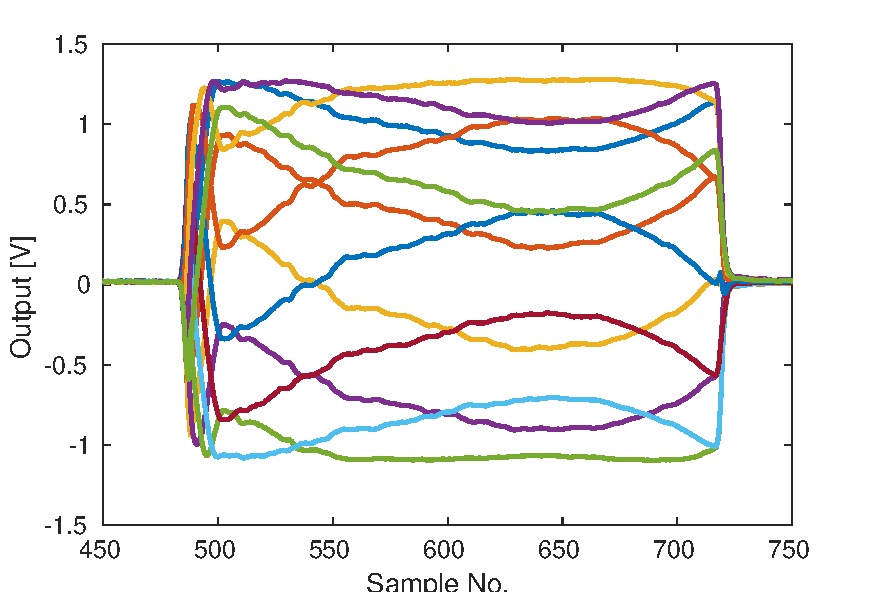
\includegraphics[width=0.9\textwidth]{Figures/phaseMons/mon1AllPoints}
  \caption{Mon~1 phase along the pulse for each LO phase shifter setting during the calibration.}
  \label{f:mon1AllPoints}
 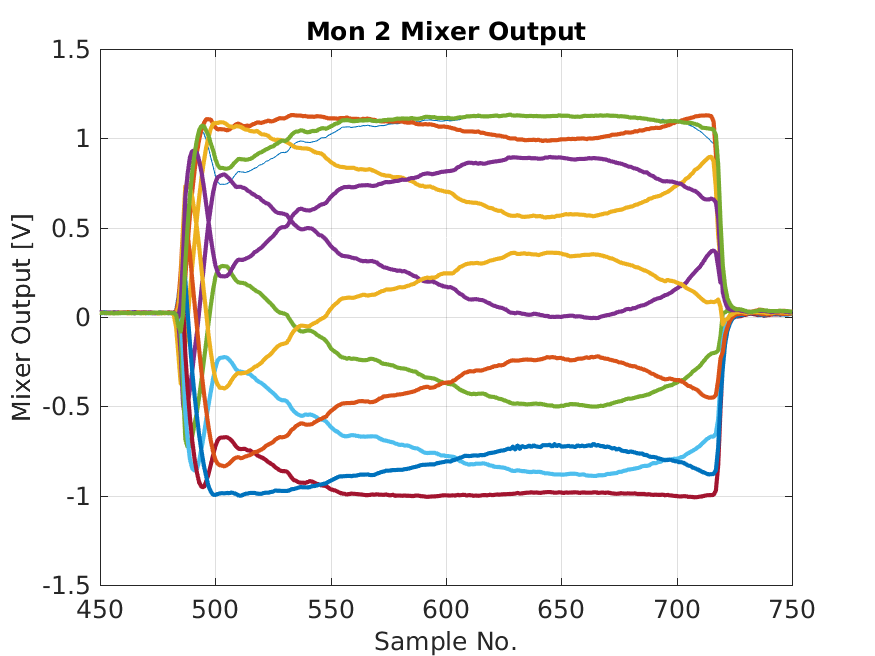
\includegraphics[width=0.9\textwidth]{Figures/phaseMons/mon2AllPoints}
  \caption{Mon~2 phase along the pulse for each LO phase shifter setting during the calibration.}
  \label{f:mon2AllPoints}
\end{figure}

\begin{figure}
  \centering
  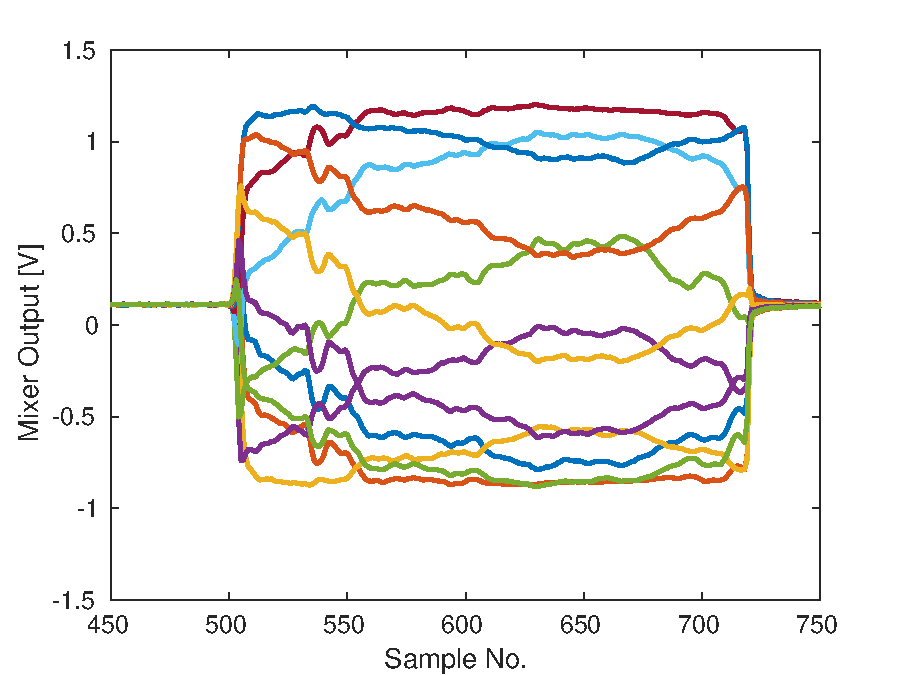
\includegraphics[width=0.9\textwidth]{Figures/phaseMons/mon3AllPoints}
  \caption{Mon~3 phase along the pulse for each LO phase shifter setting during the calibration.}
  \label{f:mon3AllPoints}
\end{figure}

Figure~\ref{f:calSiS} shows the result of fitting the mixer output versus the phase shifter setting at sample 605 along the pulse. The mixer response is sinusoidal as expected and as seen previously in the signal generator tests. In the signal generator tests there was some visible distortion away from the sine fit around the peaks at some input power levels (Section~\ref{ss:sigGenMixer}). There is no visible effect at the powers of the phase monitor signals (Section~\ref{s:phaseMonDesign}). Differences in the peak output of each monitor are expected due to differences in the input power from each phase monitor as well as differences between the sets of electronics. Small offsets between the data and the fit at some shifter settings are caused by drifts in the beam phase during the scan (particularly for Mon~3 where the beam is less stable), as well as human error in setting the shifter values.

The fitted values of the mixer amplitude, \(A\), and offset, \(d\), are found in Table~\ref{t:calSiSConsts}. These values are used to calculate the beam phase as per Equation~\ref{e:phaseRecUsed}. 

\begin{figure}
  \centering
  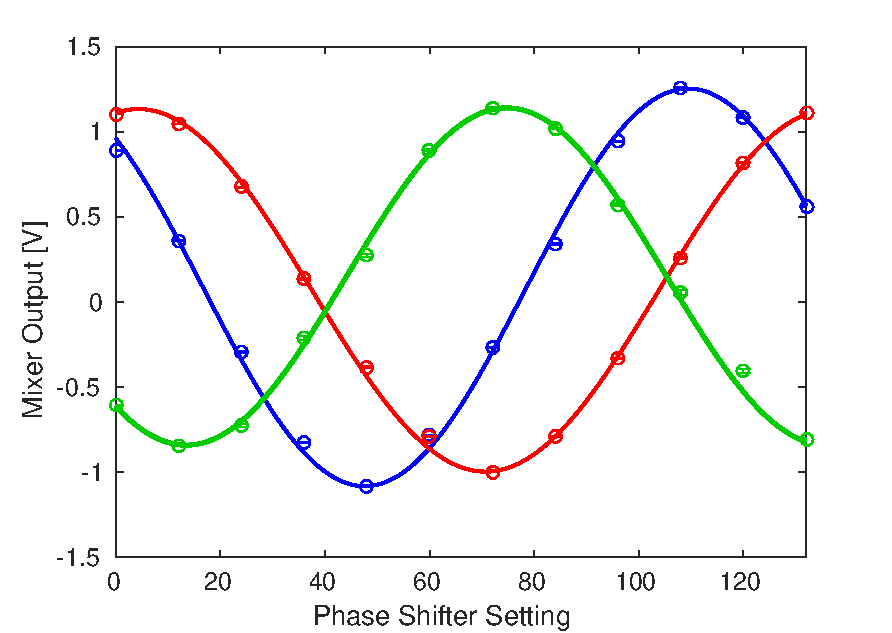
\includegraphics[width=0.9\textwidth]{Figures/phaseMons/calSiS}
  \caption{Fits to the mixer output vs. LO phase shifter setting at sample 605 on the SiS digitisers.}
  \label{f:calSiS}
\end{figure}

\begin{table}
  \begin{center}
    \begin{tabular}{|c c c|}
	   \hline
       Monitor & \(A\) (amplitude) & \(d\) (offset) \\ \hline
       Mon~1 & \(1167\pm10\)~mV & \(86\pm9\)~mV \\ 
       Mon~2 & \(1064\pm6\)~mV & \(69\pm7\)~mV\\
       Mon~3 & \(990\pm12\)~mV & \(150\pm10\)~mV\\ \hline
    \end{tabular}
    \caption{Fit parameters from the calibration on the SiS digitisers for each monitor.}
  	\label{t:calSiSConsts}
  \end{center}
\end{table}

\subsection{Calibration on FONT5a Board}
\label{ss:FONTCal}

Figure~\ref{f:calFONT} and Table~\ref{t:calFONTConsts} show the results of a calibration performed in exactly the same way but on the FONT5a board. The FONT5a board ADCs flip the sign of the input [REF], so a positive ADC output in counts corresponds to a negative input voltage and vice-versa. This explains why the apparent mixer output is on the rising slope at a phase shifter setting of zero on the FONT5a board in Figure~\ref{f:calFONT}, but on the falling slope on the SiS digitisers in Figure~\ref{f:calSiS}. For operation of the PFF system this difference must be taken in to account either by operating the mixer on the rising slope as seen on the FONT5a board (which in reality is the falling slope, as desired), or alternatively by using negative gain values for the correction output. The fitted values for \(d\) in Table~\ref{t:calFONTConsts} are also negative rather than positive as a result of this sign flip. Apart from these differences the overall shape of the mixer output follows the sinusoidal dependence as expected.

The FONT5a ADC outputs are 13-bit, or \(\pm4096\)~counts, with an input range of \(\pm500\)~mV (Section~\ref{s:fontSetup}). The fitted Mon~1 output, with 1~dB attenuation added after the mixer, of between -3712~counts and +3156~counts therefore corresponds to an input voltage range of between +453~mV and -385~mV. Without the attenuator, which reduces the voltage by roughly 10\%, the Mon~1 mixer would saturate the ADC at its peak output. As the contribution of digitiser noise is small on the FONT5a board (Section~\ref{s:monDigitisers}) a 1~dB attenuator is also added to the Mon~2 and Mon~3 outputs so that the overall setup for each monitor is the same in this measurement. However, during normal operation of the PFF system Mon~2 and Mon~3 are connected to the SiS digitisers, with their mixer outputs then being amplified rather than attenuated.

\begin{figure}
  \centering
  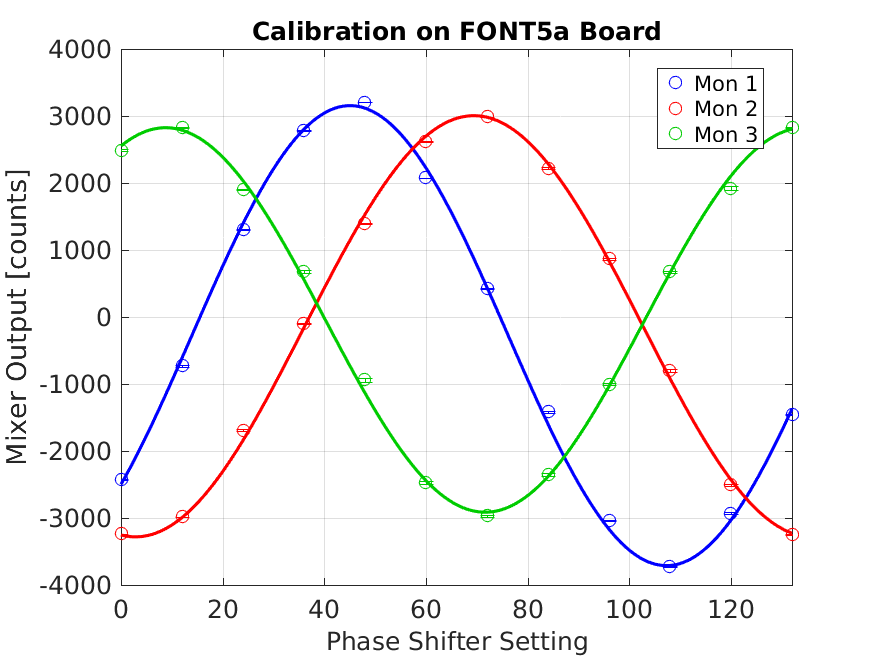
\includegraphics[width=0.9\textwidth]{Figures/phaseMons/calFONT}
  \caption{Results of a calibration performed on the FONT5a board.}
  \label{f:calFONT}
\end{figure}


\begin{table}
  \begin{center}
    \begin{tabular}{|c c c|}
	   \hline
       Monitor & \(A\) (amplitude) & \(d\) (offset) \\ \hline
       Mon~1 & \(3434\pm41\)~counts & \(-278\pm34\)~counts \\ 
       Mon~2 & \(3144\pm16\)~counts & \(-138\pm17\)~counts\\
       Mon~3 & \(2870\pm43\)~counts & \(-44\pm44\)~counts\\ \hline
    \end{tabular}
    \caption{Fit parameters from the calibration for each monitor on the FONT5a board.}
  	\label{t:calFONTConsts}
  \end{center}
\end{table}

\subsection{Multi-Sample Results}
\label{ss:calMultiSamp}

The calibration results on both the SiS digitisers and FONT5a board have been presented at one sample number around the middle of the pulse close to where the phase sag along the pulse is flattest. In this section the variation in the fitted calibration constants along the pulse is discussed. This is particularly important after taking the decision to not use the diodes, as the intended purpose of using the diodes was to normalise the mixer response to give an output independent of the input power. Without using the diodes any variations in input power along the pulse will also create differences in the calibration constants along the pulse. 

The current implementation of the PFF algorithm on the FONT5a board uses the mixer multiplied by one gain value that is constant along the full pulse length to create the correction output (Section~\ref{ss:pffFirmware}). It therefore cannot take in to account any variations in calibration constants along the pulse. Offline data analysis is usually performed in the same way so that the quoted resolutions are representative of the values that apply to the implementation of the PFF correction. The effect of taking in to account the variations in calibration parameters along the pulse seen here is shown in Section~\ref{ss:resCalAlongPulse}.

Figures~\ref{f:calAmpVsSample}~and~\ref{f:calOffVsSample} show the variation in the fitted calibration amplitude and offset across the full pulse length, using the same calibration on the SiS digitisers presented in Section~\ref{ss:SiSCal}. Differences in both the amplitude and offset along the pulse are visible. These are summarised in Table~\ref{t:calConstsStdAlong} in terms of the standard deviation of the fitted parameter values along the pulse. 

The stability of the fitted amplitude along the pulse is similar for the upstream monitors (Mon~1 and Mon~2), with a jitter of around 8~mV in both cases. As the downstream beam is less stable than the upstream beam the variations in fitted ampltidue along the pulse are larger for Mon~3, at the 15~mV level. In terms of a relative difference these values correspond to roughly a 0.7\% variation in fitted amplitude for Mon~1 and Mon~2, or 1.5\% for Mon~3. With further optimisation of the downstream beam, as documented in Chapter~\ref{c:phasePropagation}, it should be possible to achieve similar Mon~3 amplitude stability to that seen for Mon~1 and Mon~2. 

Absolute stability in the fitted offset along the pulse is similar to that of the amplitude but therefore much larger as a relative difference at the level of several percent. The variation in fitted offset along the pulse is smallest for Mon~2 at around 3~mV. For both Mon~1 and Mon~3 the variation is around a factor two larger, at 6~mV.

\begin{figure}
  \centering
  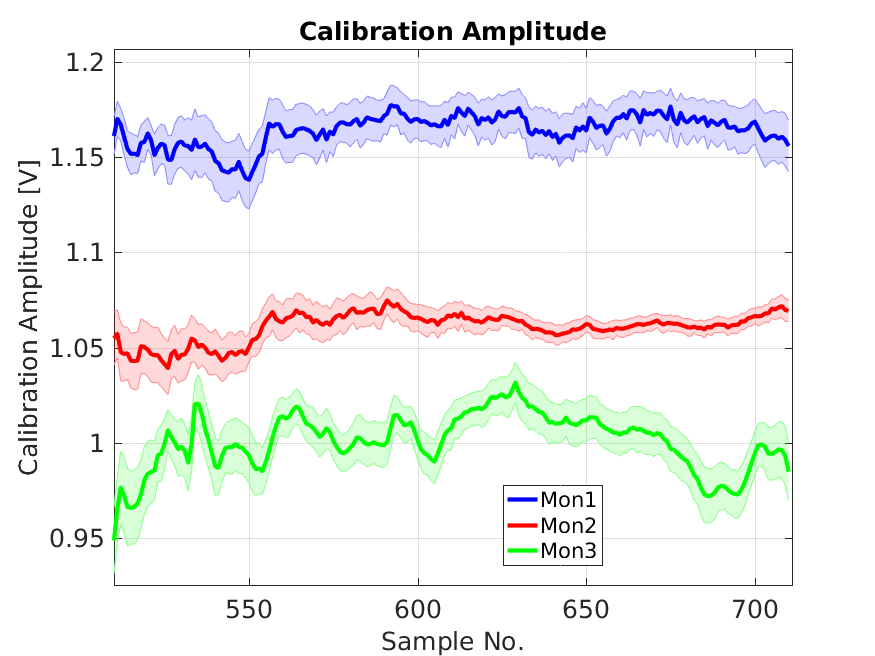
\includegraphics[width=0.9\textwidth]{Figures/phaseMons/calAmpVsSample}
  \caption{Variation in fitted amplitude along the pulse for each phase monitor.}
  \label{f:calAmpVsSample}
  \centering
  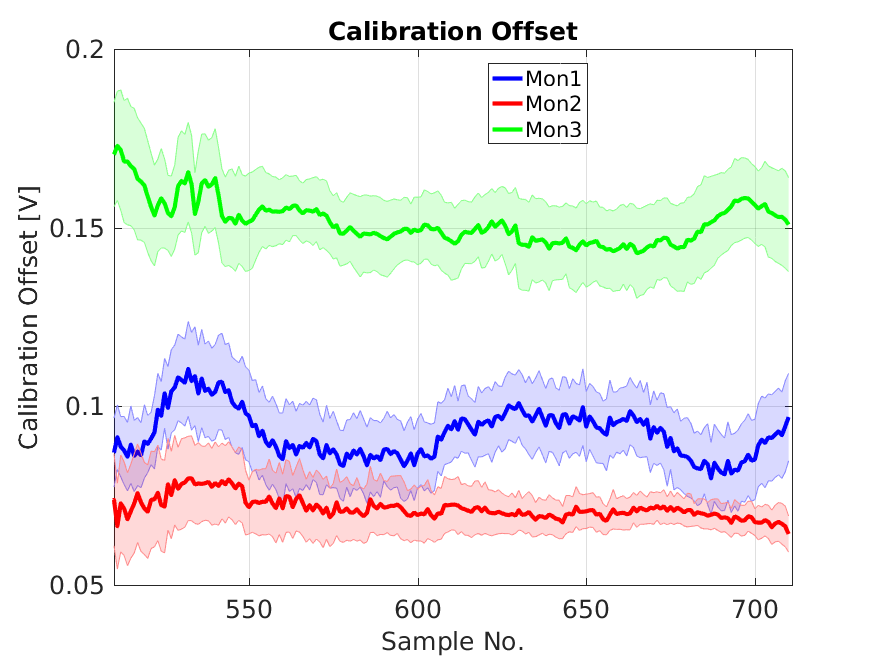
\includegraphics[width=0.9\textwidth]{Figures/phaseMons/calOffVsSample}
  \caption{Variation in fitted offset along the pulse for each phase monitor}
  \label{f:calOffVsSample}
\end{figure}

\begin{table}
  \begin{center}
    \begin{tabular}{|c c c|}
	   \hline
       Monitor & \(A\) (amplitude) & \(d\) (offset) \\ \hline
       Mon~1 & \(8.3\pm0.4\)~mV & \(6.7\pm0.3\)~mV \\ 
       Mon~2 & \(7.7\pm0.4\)~mV & \(3.0\pm0.3\)~mV\\
       Mon~3 & \(14.7\pm0.7\)~mV & \(6.1\pm0.3\)~mV\\ \hline
    \end{tabular}
    \caption{Standard deviation in calibration fit parameters along the pulse.}
  	\label{t:calConstsStdAlong}
  \end{center}
\end{table}

\subsection{Zero Crossing}
\label{ss:calZeroCross}

The full fit to the calibration result that is performed is:
\begin{equation}
\mathrm{Mixer} = A\sin(bx + c) + d
\end{equation}
Where \(x\) is the phase shifter setting. \(A\) and \(d\) are the calibration constants used to reconstruct the phase, with their values already quoted in Table~\ref{t:calFitConsts}. The remaining fit parameters \(b\) and \(c\) convert the phase shifter setting in to the phase offset between the LO and the beam. As the shifter readings are approximately in 4~GHz degrees, the expected value for \(b\) that converts the shifter value in to 12~GHz radians is \((12/4)*(\pi/180) \simeq 50\)~mrad/unit.

To obtain the best resolution for the measurement the mixers should be operated where the dependence of the output voltage on the phase is maximal. This means maximising the partial derivative of the mixer output with respect to the phase shifter setting:
\begin{equation}
\frac{\partial \mathrm{Mixer}}{\partial x} = Ab\cos(bx+c)
\end{equation}
This is maximised when \(bx + c = n\pi\), where \(n\) is any positive or negative integer. The optimal phase shifter settings therefore meet this criteria:
\begin{equation}
x = \frac{n\pi-c}{b}
\end{equation}
Where the mixer output is \(\mathrm{Mixer} = A\sin(n\pi)+d = d\). In the case where there is no offset between the minimum and maximum mixer output (\(d=0\)) the optimal point to operate the mixers is at zero output. Because of this the optimal shifter setting will be referred to as the zero crossing. In reality the small asymmetry in the mixer output means the optimal shifter setting is where mixer output is \(d\). The effect of operating the mixers away from the zero crossing on the resolution is shown in Section~\ref{s:resVsShifter}.

In addition, as previously mentioned the convention is to operate the mixers on the falling slope where the partial derivate above is negative. The set shifter values are obtained using the smallest positive integer \(n\) that leads to this criteria being met. Table~\ref{t:calZeroCross} shows an example of values for the fit parameters \(b\) and \(c\) and the calculated phase shifter settings to be on the zero crossing for each monitor. These values are taken from the same calibration and sample number presented in Section~\ref{ss:SiSCal} (on the SiS digitisers). The reader may be interested to compare where the shifter settings fall along the mixer output traces during the calibration in Figure~\ref{f:allMixersSamp605}.

\begin{table}
  \begin{center}
    \begin{tabular}{|c c c c|}
	   \hline
       Monitor & \(b\) & \(c\) & Zero Crossing \\ \hline
       Mon~1 & \(50.8\pm0.5\)~mrad/unit & \(2.29\pm0.04\)~rad & \(16.7\pm0.9\)~units \\ 
       Mon~2 & \(47.4\pm0.5\)~mrad/unit & \(1.36\pm0.04\)~rad & \(37.5\pm0.8\)~units \\
       Mon~3 & \(51.3\pm0.6\)~mrad/unit & \(4.02\pm0.04\)~rad & \(105.5\pm1.5\)~units \\ \hline
    \end{tabular}
    \caption{Phase shifter setting to obtain the zero crossing for each mixer output and the fit parameters needed to calculate them.}
  	\label{t:calZeroCross}
  \end{center}
\end{table}

Due to the large phase sag along the beam pulse it is clearly not possible to be at the zero crossing of the mixer for the full pulse length. For the PFF system the region of interest is the central portion of the pulse where the phase sag is flattest. The shifters are therefore set to zero the mixer output in this region, giving best resolution in the central part of the pulse but degraded resolution near the start and end of the pulse. In addition to this, slow drifts in the beam phase, particularly downstream, mean that the shifters must routinely be changed to stay at the zero crossing. With the current setup using mechanical phase shifters this must be done by hand, with no possibility to implement an automatic feedback on the shifter settings, for example.



\newsection{shifters}{Phase Shifter Noise}

\begin{figure}
  \centering
  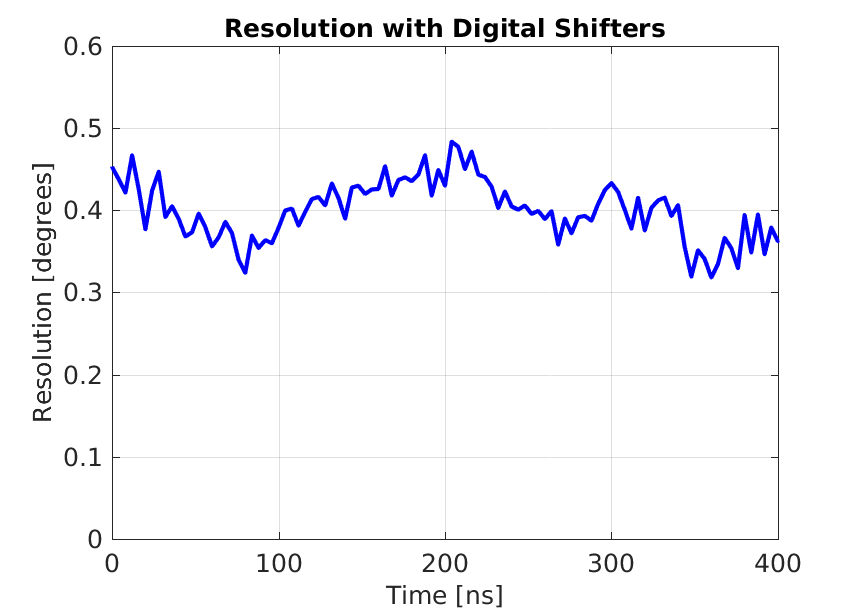
\includegraphics[width=0.9\textwidth]{Figures/phaseMons/resolutionDigShift}
  \caption{Phase monitor resolution using initial setup with digital phase shifters in place.}
  \label{f:resolutionDigShift}
\end{figure}

\begin{figure}
  \centering
  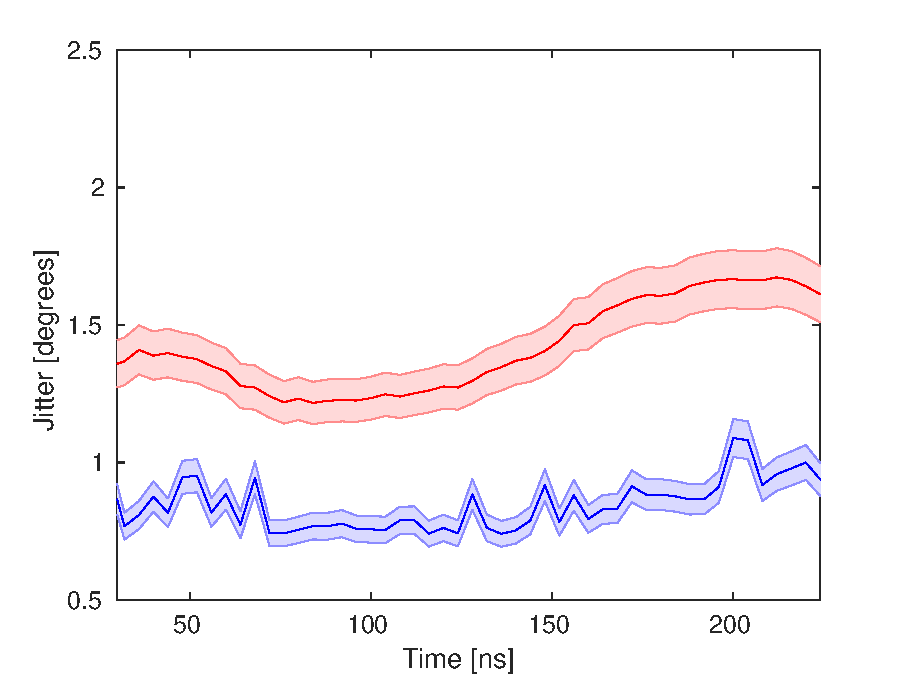
\includegraphics[width=0.9\textwidth]{Figures/phaseMons/Mix1Mon1_Mix2Mon2}
  \caption{Phase jitter along the pulse with the nominal electronics setup -- Mon~1 connected to the first mixer, and Mon~2 connected to the second mixer.}
  \label{f:Mix1Mon1_Mix2Mon2}
\end{figure}

\begin{figure}
  \centering
  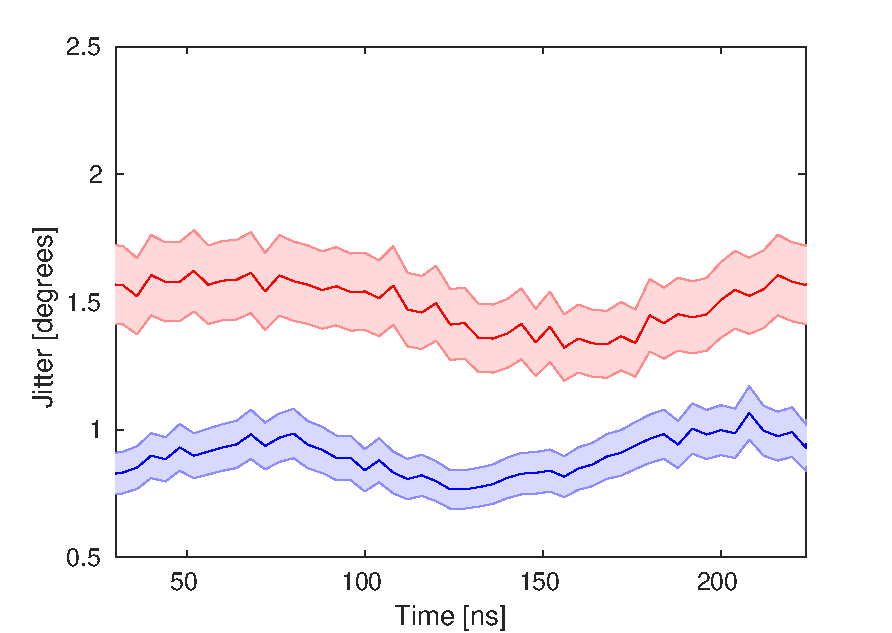
\includegraphics[width=0.9\textwidth]{Figures/phaseMons/Mix1Mon2_Mix2Mon1}
  \caption{Phase jitter along pulse with Mon~2 connected to the first mixer and Mon~1 connected to the second mixer.}
  \label{f:Mix1Mon2_Mix2Mon1}
\end{figure}

\begin{figure}
  \centering
  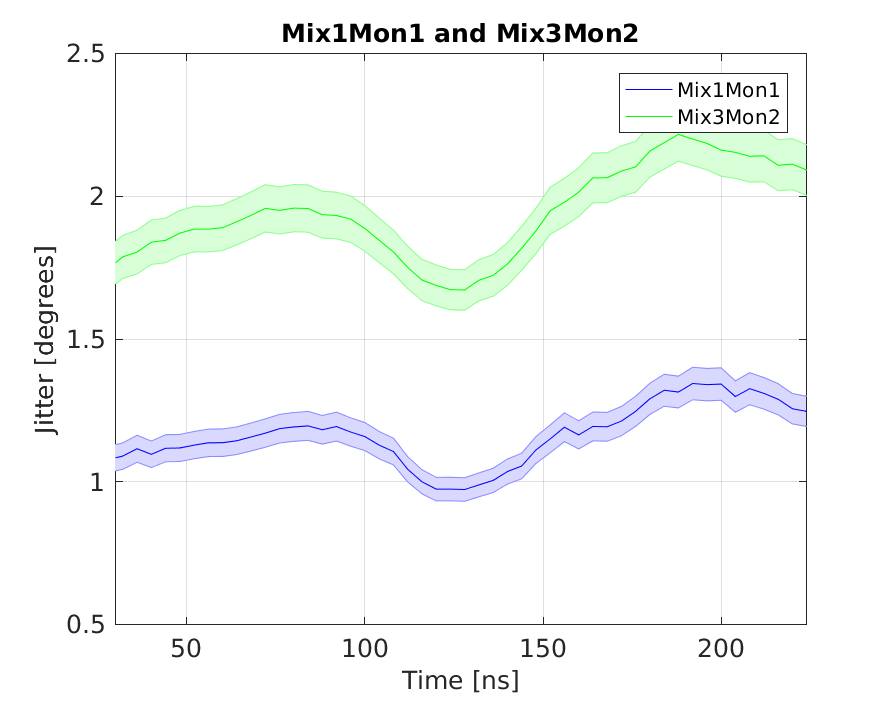
\includegraphics[width=0.9\textwidth]{Figures/phaseMons/Mix1Mon1_Mix3Mon2}
  \caption{Phase jitter along pulse with Mon~1 connected to the first mixer and Mon~2 connected to the third mixer.}
  \label{f:Mix1Mon1_Mix3Mon2}
\end{figure}

\begin{figure}
  \centering
  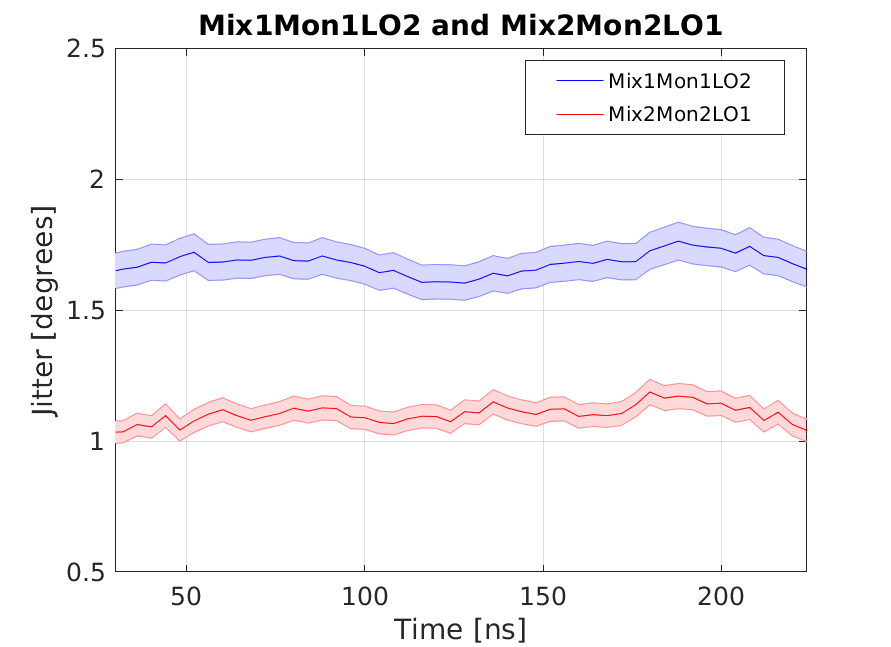
\includegraphics[width=0.9\textwidth]{Figures/phaseMons/Mix1Mon1PhShft2_Mix2Mon2PhShft1}
  \caption{Phase jitter along pulse with the phase shifters swapped between the first mixer and the second mixer.}
  \label{f:Mix1Mon1PhShft2_Mix2Mon2PhShft1}
\end{figure}

\begin{figure}
  \centering
  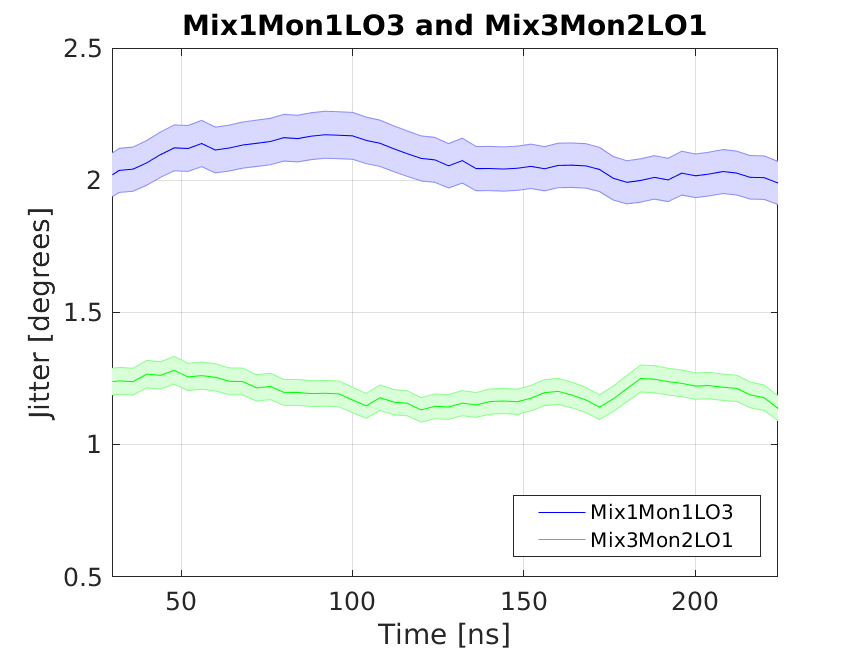
\includegraphics[width=0.9\textwidth]{Figures/phaseMons/Mix1Mon1PhShft3_Mix3Mon2PhShft1}
  \caption{Phase jitter along pulse with the phase shifters swapped between the third mixer and the first mixer.}
  \label{f:Mix1Mon1PhShft3_Mix3Mon2PhShft1}
\end{figure}

\begin{table}
  \begin{center}
    \begin{tabular}{|c c c | c c c|}
	   \hline
	   & Mon~1 & & & Mon~2 & \\ \hline
      Mixer & Shifter & Jitter & Mixer & Shifter & Jitter \\ \hline
      1 & \textbf{1} & \(\mathbf{0.83\pm0.01^\circ}\) & 2 & 2 & \(1.38\pm0.01^\circ\)    \\
      2 & 2 & \(1.48\pm0.02^\circ\) & 1 & \textbf{1} & \(\mathbf{0.89\pm0.01^\circ}\)    \\ 
      1 & \textbf{1} & \(\mathbf{1.15\pm0.01^\circ}\) & 3 & 3 & \(1.91\pm0.01^\circ\)    \\ 
      1 & 2 & \(1.68\pm0.01^\circ\) & 2 & \textbf{1} & \(\mathbf{1.10\pm0.01^\circ}\)    \\ 
      1 & 3 & \(2.07\pm0.01^\circ\) & 3 & \textbf{1} & \(\mathbf{1.20\pm0.01^\circ}\)    \\  
	\hline
    \end{tabular}
    \caption{Comparison of phase jitter along the pulse for each measurement with different setups of the electronics. Each row corresponds to the results of one dataset. The left hand side of the table shows the results from Mon~1 in that dataset, and the right hand side of the table the results from Mon~2. Bold text indicates the lower jitter value in that dataset, all of which use the first phase shifter.}
  	\label{t:elecSwapResults}
  \end{center}
\end{table}

\begin{figure}
  \centering
  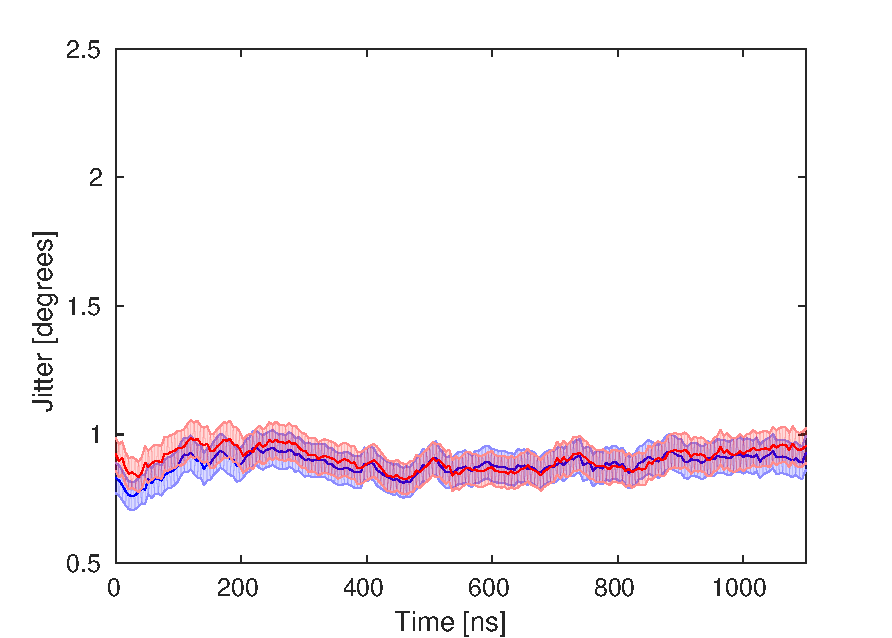
\includegraphics[width=0.9\textwidth]{Figures/phaseMons/jitterMechanicalShifters}
  \caption{Phase jitter along pulse after installation of the mechanical phase shifters.}
  \label{f:jitterMechanicalShifters}
\end{figure}


\newsection{resolutionMeas}{Resolution Measurements}

\subsection{Best Resolution}
\label{ss:bestRes}

Mean is \(0.1257\pm0.0005^\circ\) 

\begin{figure}
  \centering
  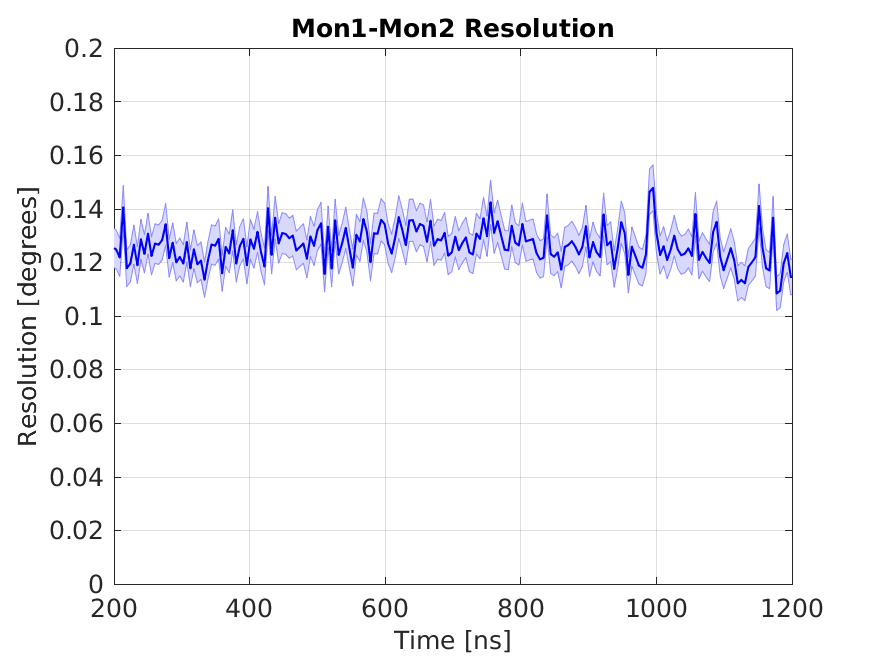
\includegraphics[width=0.9\textwidth]{Figures/phaseMons/bestResolution}
  \caption{bestResolution}
  \label{f:bestResolution}
\end{figure}

\subsection{With Sample Averaging}
\label{ss:resCalAlongPulse}

\(0.1077\pm0.0005^\circ\) with 5 samples averaged

\begin{figure}
  \centering
  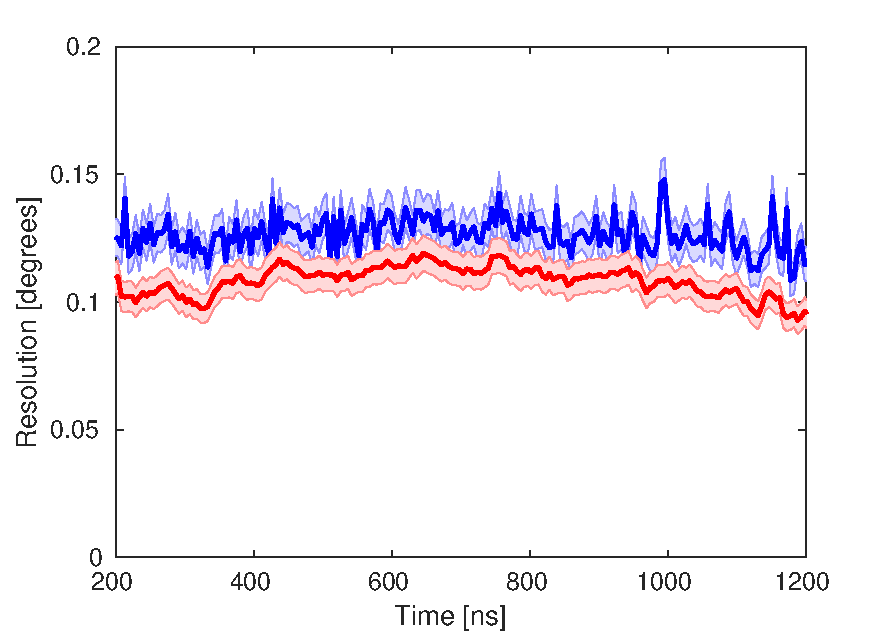
\includegraphics[width=0.9\textwidth]{Figures/phaseMons/resolutionWithAveraging}
  \caption{Effect on resolution by averaging samples.}
  \label{f:resolutionWithAveraging}
\end{figure}


\subsection{Dependence of Resolution on LO Phase}
\label{ss:resVsShifter}

The process of setting the mixers on their zero crossing after calibrations was documented in Section~\ref{ss:calZeroCross}. This is necessary to operate the mixers where there output voltage is most sensitive to variations in the phase (close to the peaks of the mixer output there is negligible change in output voltage for small changes in phase). The dependence of the phase resolution on the beam phase across the full \(\pm180^\circ\) range is shown in Figure~\ref{f:resolutionVsShifter}. The plotted phase is the offset between the LO phase shifter setting and the calculated optimal setting. More than \(50^\circ\) away from the zero crossing there is a large degradation in resolution, reaching above 1~degree at the \(+90^\circ\) peak.

However, for the PFF system the phase resolution only needs to be guaranteed within its correction range, which is close to \(\pm6^\circ\) as seen in Section~\ref{ss:corrRange}. In Figure~\ref{f:resVsSmallPhasOff} it is seen that there is no noticeable degradation in resolution in the range between \(\pm15^\circ\).

\begin{figure}
  \centering
  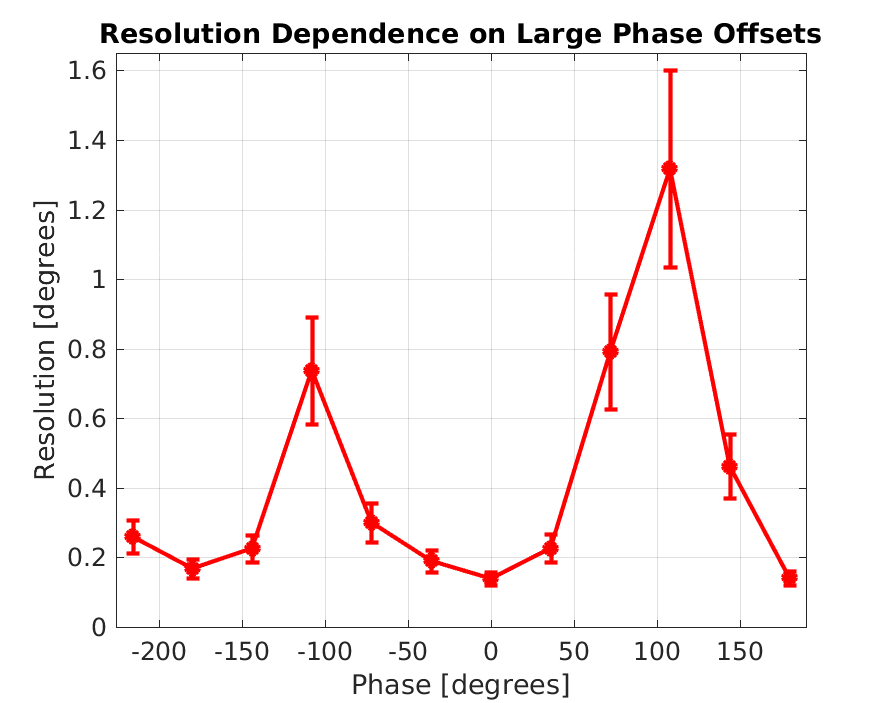
\includegraphics[width=0.9\textwidth]{Figures/phaseMons/resolutionVsShifter}
  \caption{Resolution.}
  \label{f:resolutionVsShifter}
  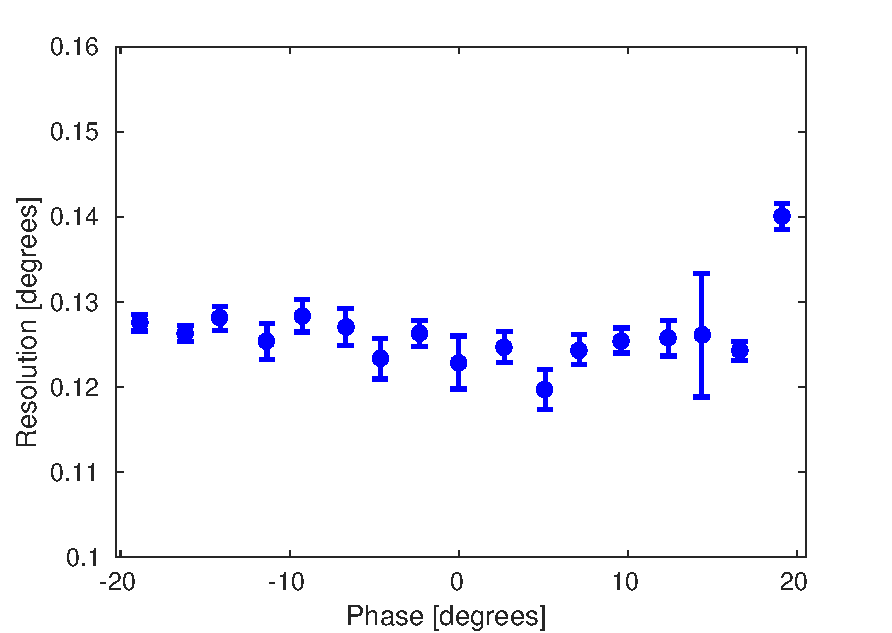
\includegraphics[width=0.9\textwidth]{Figures/phaseMons/resVsSmallPhasOff}
  \caption{Resolution.}
  \label{f:resVsSmallPhasOff}
\end{figure}

\subsection{Dependence of Resolution on Input Power}
\label{ss:resVsPower}

Would need to take new data to do this section properly. Have some data with input attenuation 0dB 10dB 13dB 16dB 20dB but from before new shifters (with adjusters), and really need more in the range from 0dB to 10dB rather than at very high attenuations.

\newsection{monComp}{Differences Between Monitors}

shape mon1 vs mon2
jitter mon1 vs mon2
comparison mon1/2 and bpr
comparison mon3 and pets

\begin{figure}
  \centering
  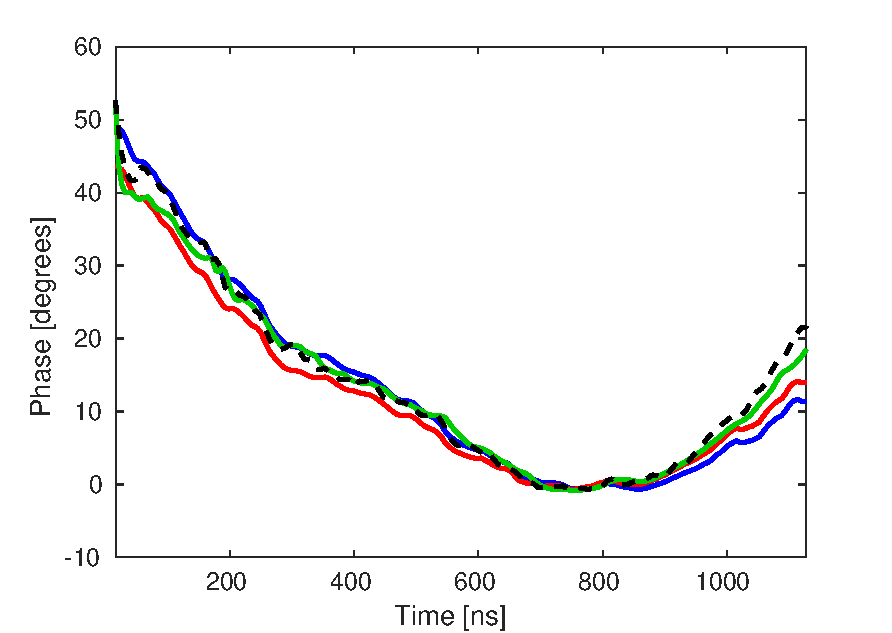
\includegraphics[width=0.9\textwidth]{Figures/phaseMons/phaseAlongAll}
  \caption{Comparison of phase along the pulse in the three PFF phase monitors and an alternative phase measurement from a PETS.}
  \label{f:phaseAlongAll}
\end{figure}


\begin{figure}
  \centering
  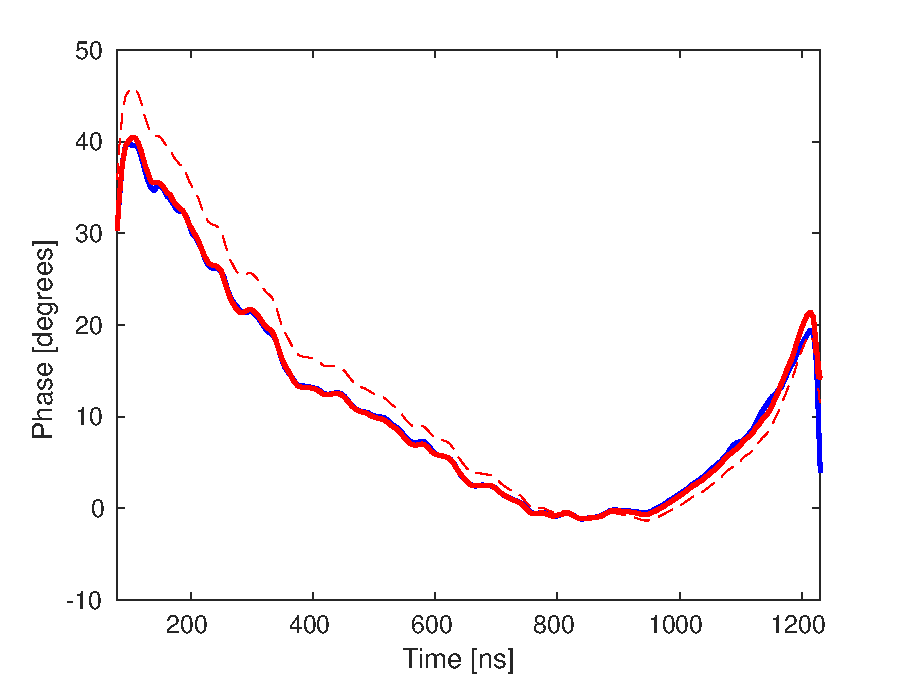
\includegraphics[width=0.8\textwidth]{Figures/phaseMons/mon2Rotated}
  \caption{Comparison of Mon~1 and Mon~2 phase along the pulse, with Mon~2 rotated by \(2.1^\circ\) about a time of 850~ns on the horizontal axis.}
  \label{f:mon2Rotated}
  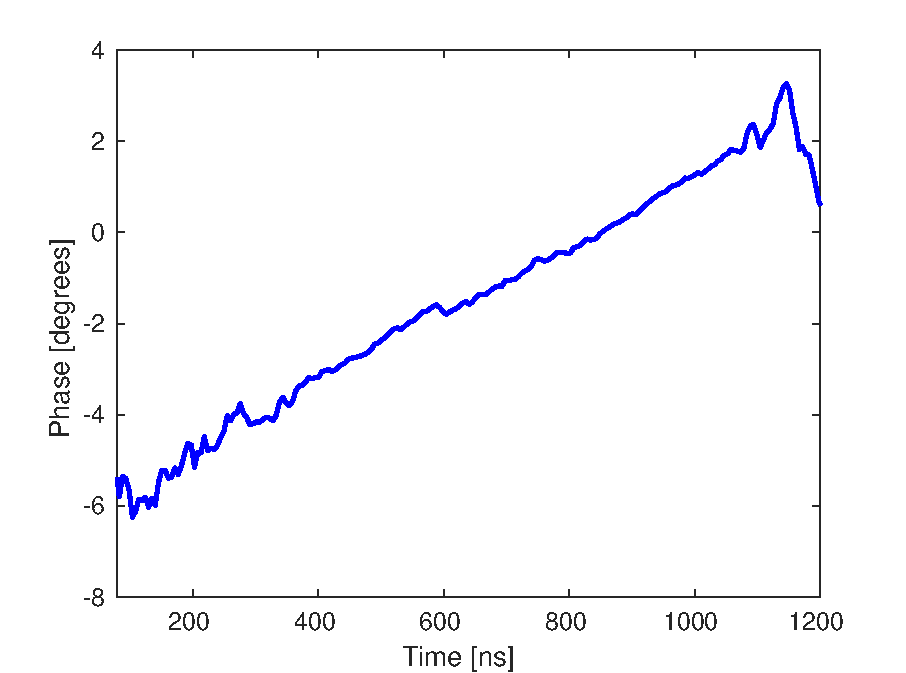
\includegraphics[width=0.8\textwidth]{Figures/phaseMons/DiffMon1Mon2Along}
  \caption{Difference between Mon~1 and Mon~2 phase along the pulse with and without Mon~2 rotated.}
  \label{f:DiffMon1Mon2Along}
\end{figure}

rotation reduces \(1.44\pm0.08^\circ\) mean absolute offset to \(0.12\pm0.01^\circ\) between 370~ns and 1080~ns

\newsection{effectsMultiSampCal}{Effect of Variations in Calibration Constant}


\begin{figure}
  \centering
  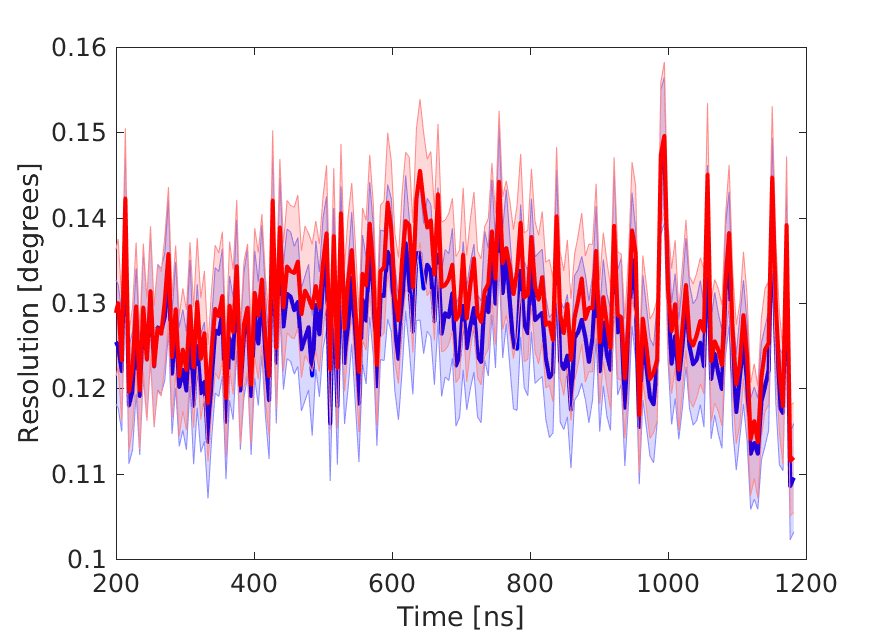
\includegraphics[width=0.9\textwidth]{Figures/phaseMons/resolutionWithMultiSampleCal}
  \caption{Effect of using a varying calibration constant on the phase resolution.}
  \label{f:resolutionWithMultiSampleCal}
\end{figure}

\begin{figure}
  \centering
  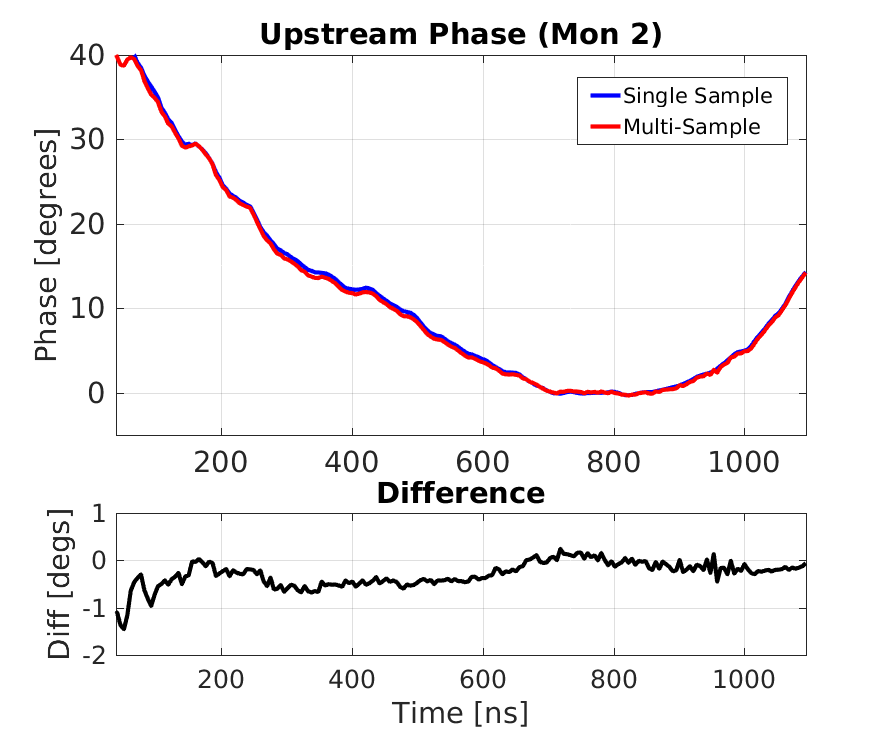
\includegraphics[width=0.9\textwidth]{Figures/phaseMons/multiSampMon2Along}
  \caption{Effect of using a varying calibration constant on the upstream phase.}
  \label{f:multiSampMon2Along}
\end{figure}

\begin{figure}
  \centering
  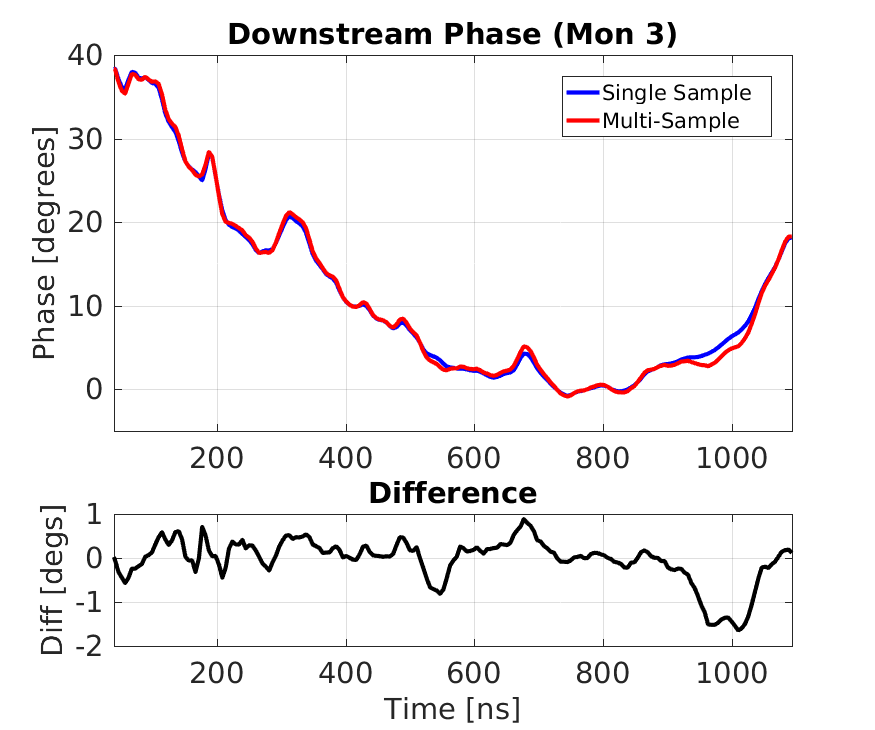
\includegraphics[width=0.9\textwidth]{Figures/phaseMons/multiSampMon3Along}
  \caption{Effect of using a varying calibration constant on the downstream phase.}
  \label{f:multiSampMon3Along}
\end{figure}

\newsection{monBandwidth}{Bandwidth}

bandwidth [GHz] is 0.35/ 10\%-90\% rise time[ns]

feature in middle goes from 156.6 ns to 167 ns: 10.4 ns, 33.7~MHz (but just 2 samples)
falling slope goes from 287 to 297 ns, suggests 35~MHz bandwidth
but pretty slow sampling rate...


\begin{figure}
  \centering
  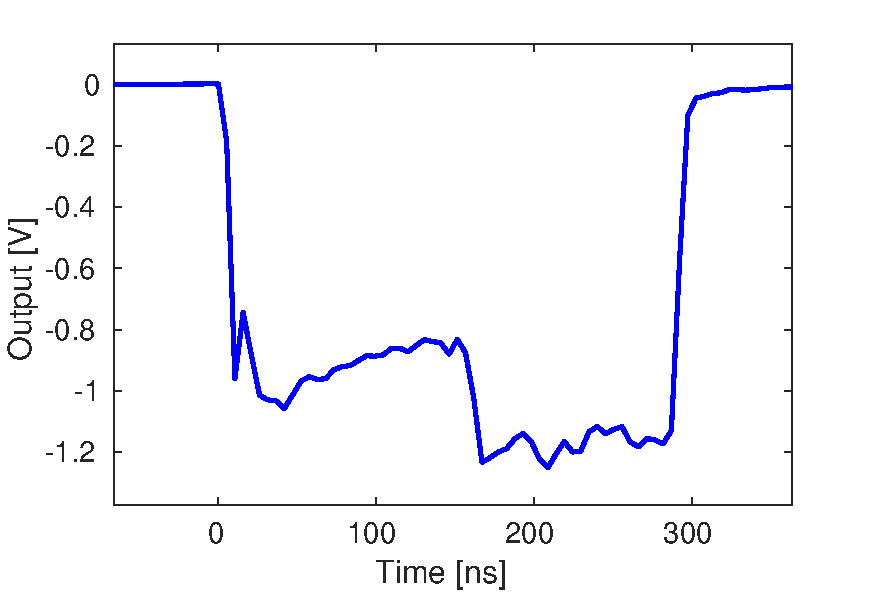
\includegraphics[width=0.9\textwidth]{Figures/phaseMons/bandwidthPlot}
  \caption{Response of Mixer~3 to a jump in phase in the middle of the pulse.}
  \label{f:bandwidthPlot}
\end{figure}

or use transient start of upstream pulse
on FONT5a board goes 30 to 41 ns, suggests 32~MHz

\begin{figure}
  \centering
  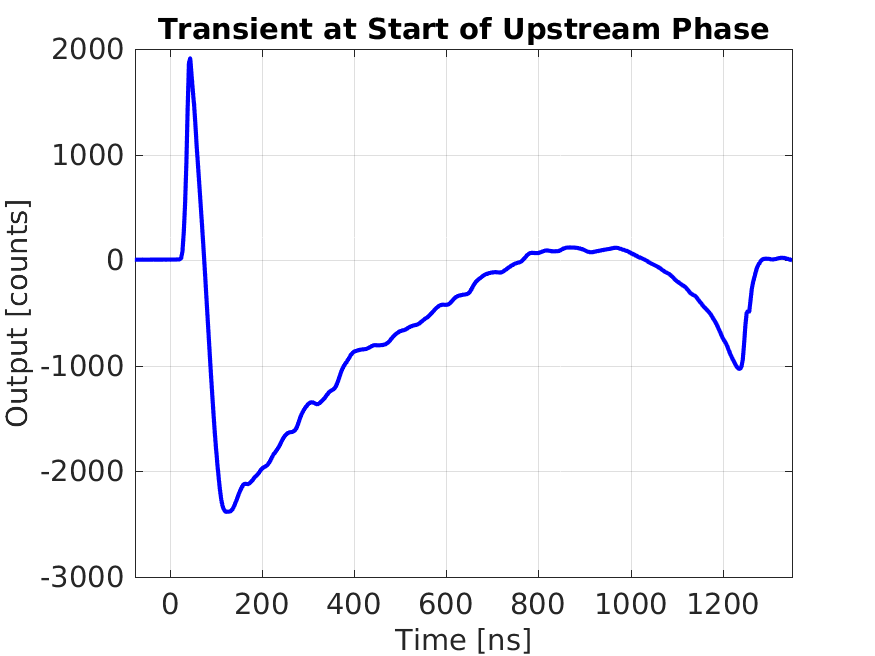
\includegraphics[width=0.9\textwidth]{Figures/phaseMons/transientUpstream}
  \caption{Energy transient at the start of the upstream pulse as seen on the second mixer.}
  \label{f:transientUpstream}
\end{figure}


\newsection{monPosition}{Dependence on Position}


\begin{table}
  \begin{center}
    \begin{tabular}{|c c c|}
	   \hline
       Device & Distance From CT.0360 & Label\\ \hline
       Mon~1 & 104.5~cm & \(s_{M1}\)\\ 
       Mon~2 & 144.5~cm & \(s_{M2}\)\\
       CT.BPM0430 & 357.0~cm & \(s_{430}\) \\ \hline
    \end{tabular}
    \caption{Distance of the upstream phase monitors and following BPM CT.0430 to the corrector CT.0360 before the phase monitors.}
  	\label{t:distanceFromCT360}
  \end{center}
\end{table}

offset in phase mons per unit offset measured in bpm 430 as result of kick in 360
\begin{align}
r_1 &= \frac{s_{M1}}{s_{430}} \\
r_2 &= \frac{s_{M2}}{s_{430}}
\end{align}
substituting in values from table gives \(r_1 = 0.29\), \(r_2 = 0.41\)

position in monitors dependent on position in 430
\begin{align}
x_{M1} &= r_{1}x_{430} \\
x_{M2} &= r_{2}x_{430}
\end{align}

mon1 and mon2 should measure same phase \(\phi_b\)
\begin{align}
\phi_{M1} &= \phi_b + c_1x_{M1} \\
\phi_{M2} &= \phi_b + c_2x_{M2}
\end{align}
\(c_1\) and \(c_2\) are phase shift per unit position offset

drifts make raw scan results look crap, so use difference between mon1 and mon2 instead
\begin{equation}
\phi_{M2}-\phi_{M1} = c_2x_{M2} - c_1x_{M1} \\
\end{equation}
have to make approximation that strength of position dependence is the same in mon1 and mon2 here to get a meaningful result \(c_1 = c_2 = c\)
\begin{align}
\phi_{M2}-\phi_{M1} &= c(x_{M2}-x_{M1}) \\
c = &\frac{\phi_{M2}-\phi_{M1}}{x_{M2}-x_{M1}} 
\end{align}
substitute in expressions for \(x_{M1}\) and \(x_{M2}\)
\begin{equation}
c = \frac{\phi_{M2}-\phi_{M1}}{x_{430}(r_2-r_1)}
\end{equation}
and \((\phi_{M2}-\phi_{M1})/x_{430}\) is gradient of fit to scan results

Horizontal
Fitted gradient phase diff vs. ct.430 is \(-0.22\pm0.01^\circ\)/mm
corresponds to phase dependence of \(-1.86\pm0.07^\circ\)/mm

Vertical
Fitted gradient phase diff vs. ct.430 is \(0.06\pm0.01^\circ\)/mm
corresponds to phase dependence of \(0.47\pm0.07^\circ\)/mm

horizontal and vertical orbit jitter looks to be at around 0.02 mm level (within factor 2?). this would give phase jitter 0.04 degrees in horizontal, 0.01 degrees in vertical

would be larger for mon3 - needs investigating
calibration will change if orbit changes

\begin{figure}
  \centering
  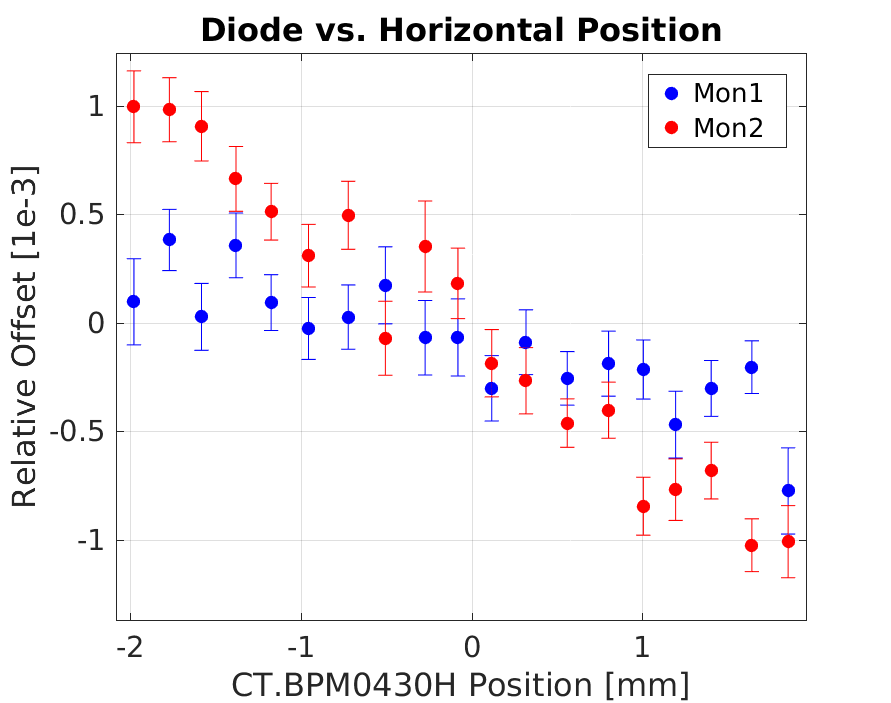
\includegraphics[width=0.9\textwidth]{Figures/phaseMons/horizontalScanDiode}
  \caption{Mon~1 and Mon~2 diode dependence on horizontal position during scan.}
  \label{f:horizontalScanDiode}
\end{figure}

\begin{figure}
  \centering
  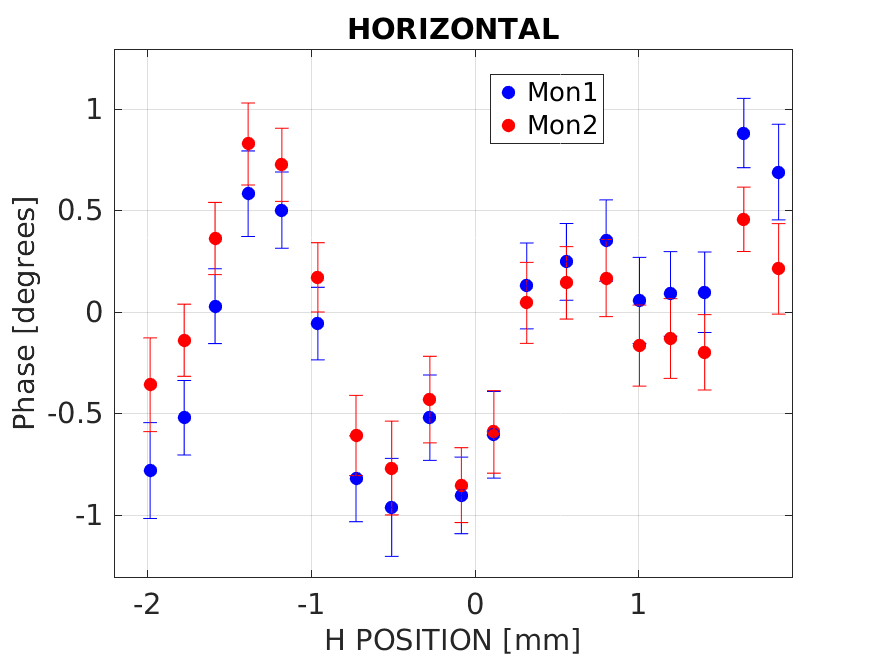
\includegraphics[width=0.9\textwidth]{Figures/phaseMons/horizontalPosScan}
  \caption{Mon~1 and Mon~2 phase dependence on horizontal position during scan.}
  \label{f:horizontalPosScan}
\end{figure}

\begin{figure}
  \centering
  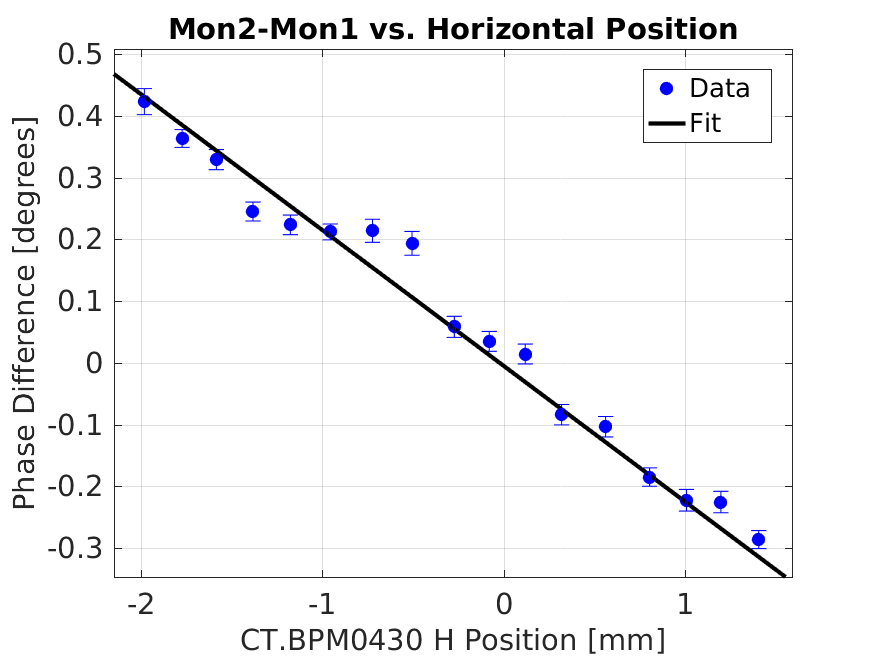
\includegraphics[width=0.9\textwidth]{Figures/phaseMons/horizontalScanFit}
  \caption{Fit to difference between Mon~1 and Mon~2 phase versus horizontal position.}
  \label{f:horizontalScanFit}
\end{figure}

\begin{figure}
  \centering
  \includegraphics[width=0.9\textwidth]{Figures/phaseMons/verticalScanFit}
  \caption{Mon~1 and Mon~2 dependence on horizontal position during scan.}
  \label{f:verticalScanFit}
\end{figure}